%!TEX root = ../main.tex
\chapter{Timing: Additional Plots}
\label{appendix:TimingAdd}

\begin{figure}[htbp!]
  \begin{subfigure}[t]{0.49\textwidth}
    \centering
    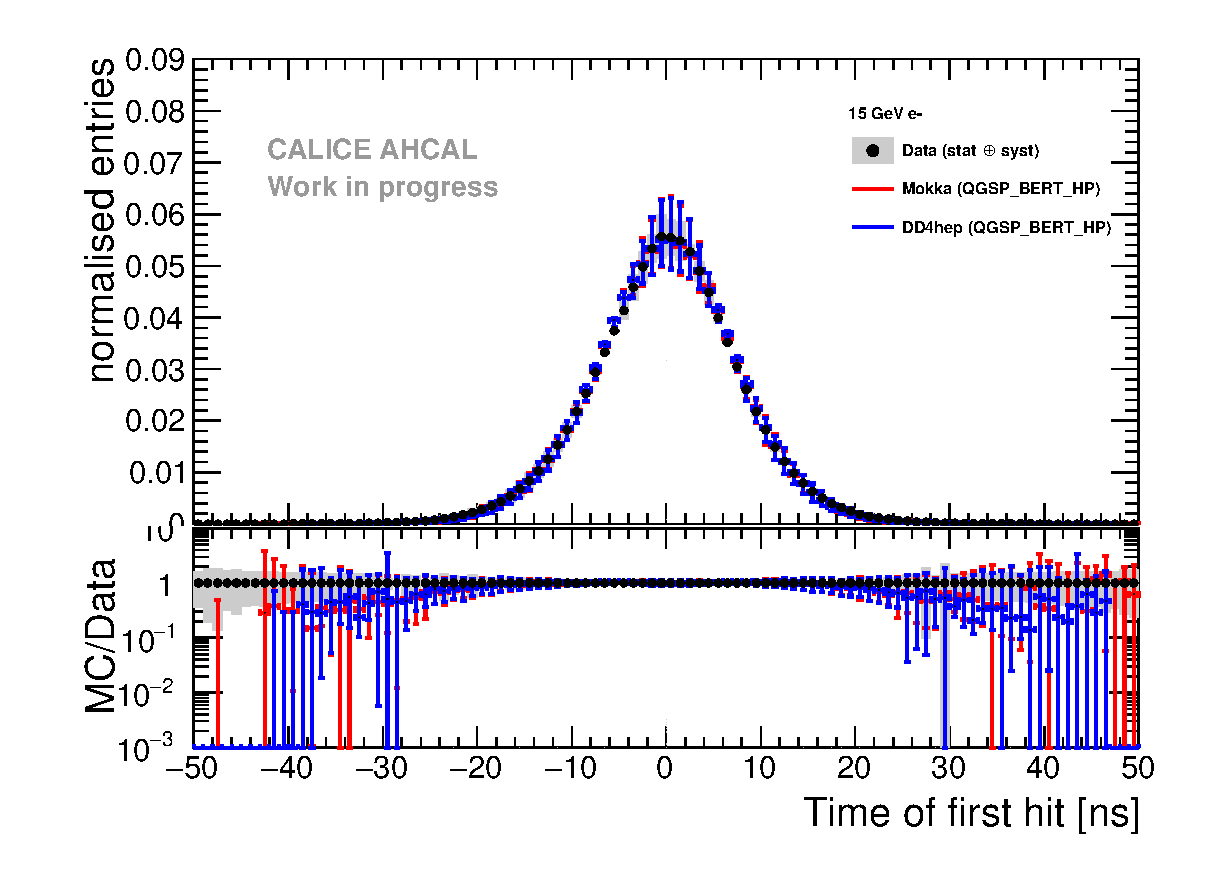
\includegraphics[width=1\textwidth]{../Thesis_Plots/Timing/Electrons/Plots/Comparison_SimData_Electrons15GeV.eps}
    \caption{15 GeV.}\label{fig:elec_sim_data_15GeV}
  \end{subfigure}
  \hfill
  \begin{subfigure}[t]{0.49\textwidth}
    \centering
    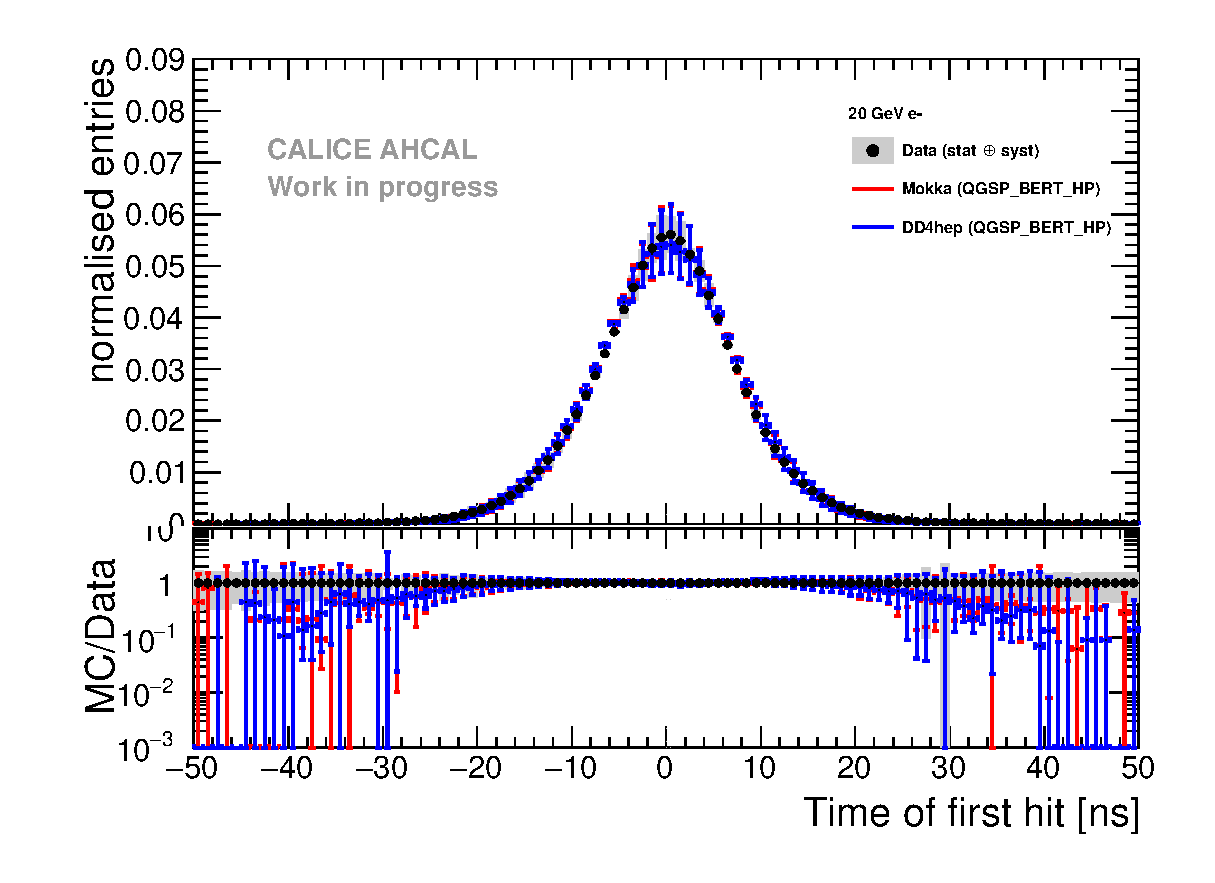
\includegraphics[width=1\textwidth]{../Thesis_Plots/Timing/Electrons/Plots/Comparison_SimData_Electrons20GeV.eps}
    \caption{20 GeV.}\label{fig:elec_sim_data_20GeV}
  \end{subfigure}
  \hfill
  \begin{subfigure}[t]{0.49\textwidth}
    \centering
    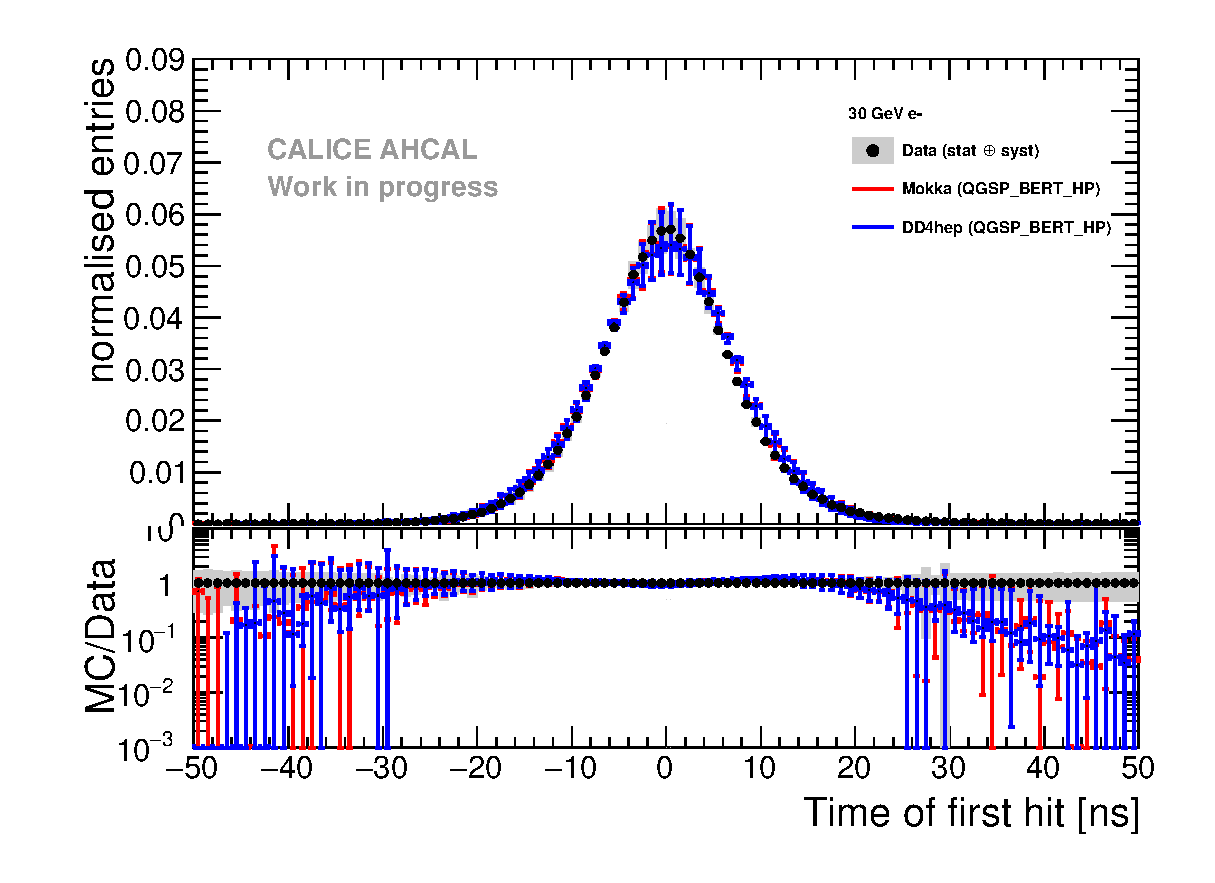
\includegraphics[width=1\textwidth]{../Thesis_Plots/Timing/Electrons/Plots/Comparison_SimData_Electrons30GeV.eps}
    \caption{30 GeV.}\label{fig:elec_sim_data_30GeV}
  \end{subfigure}
  \hfill
  \begin{subfigure}[t]{0.49\textwidth}
    \centering
    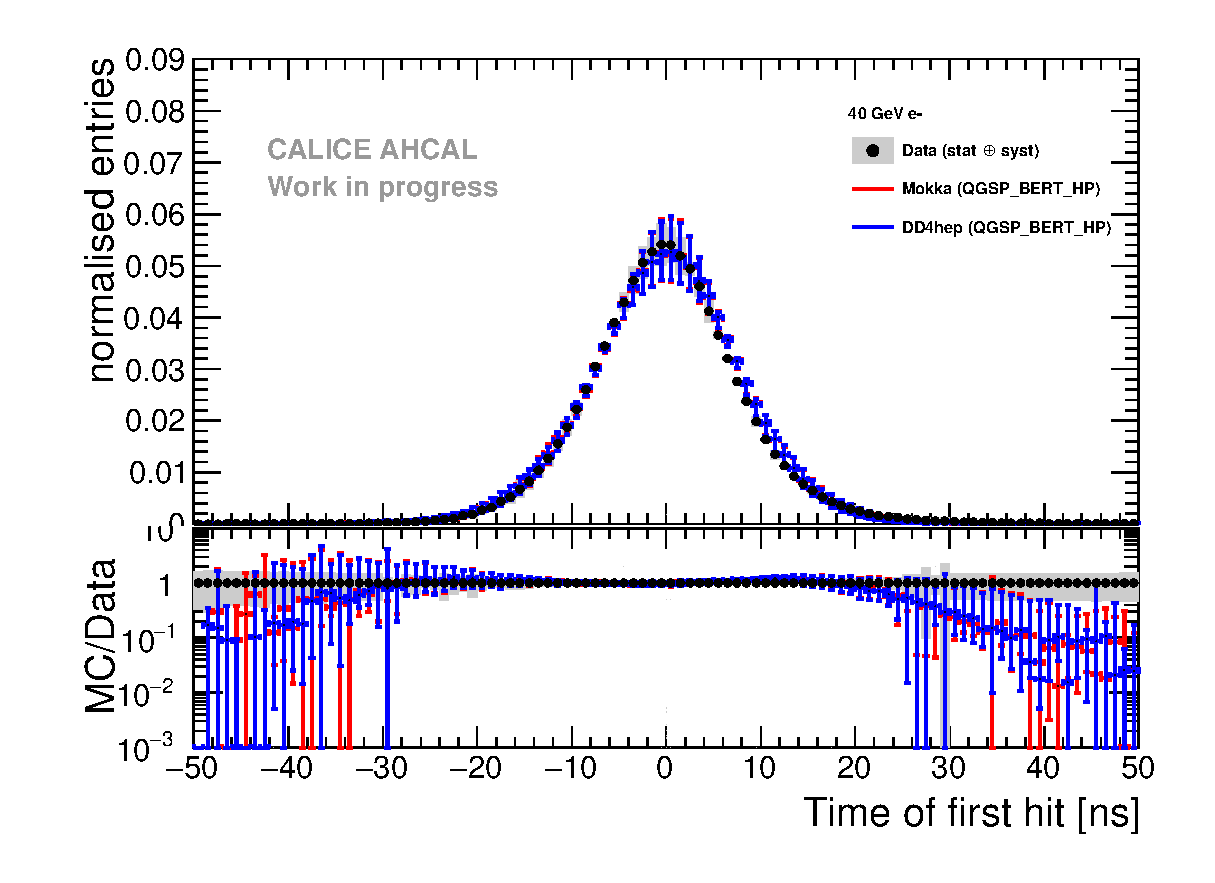
\includegraphics[width=1\textwidth]{../Thesis_Plots/Timing/Electrons/Plots/Comparison_SimData_Electrons40GeV.eps}
    \caption{40 GeV.}\label{fig:elec_sim_data_40GeV}
  \end{subfigure}
  \hfill
  \begin{subfigure}[t]{0.49\textwidth}
    \centering
    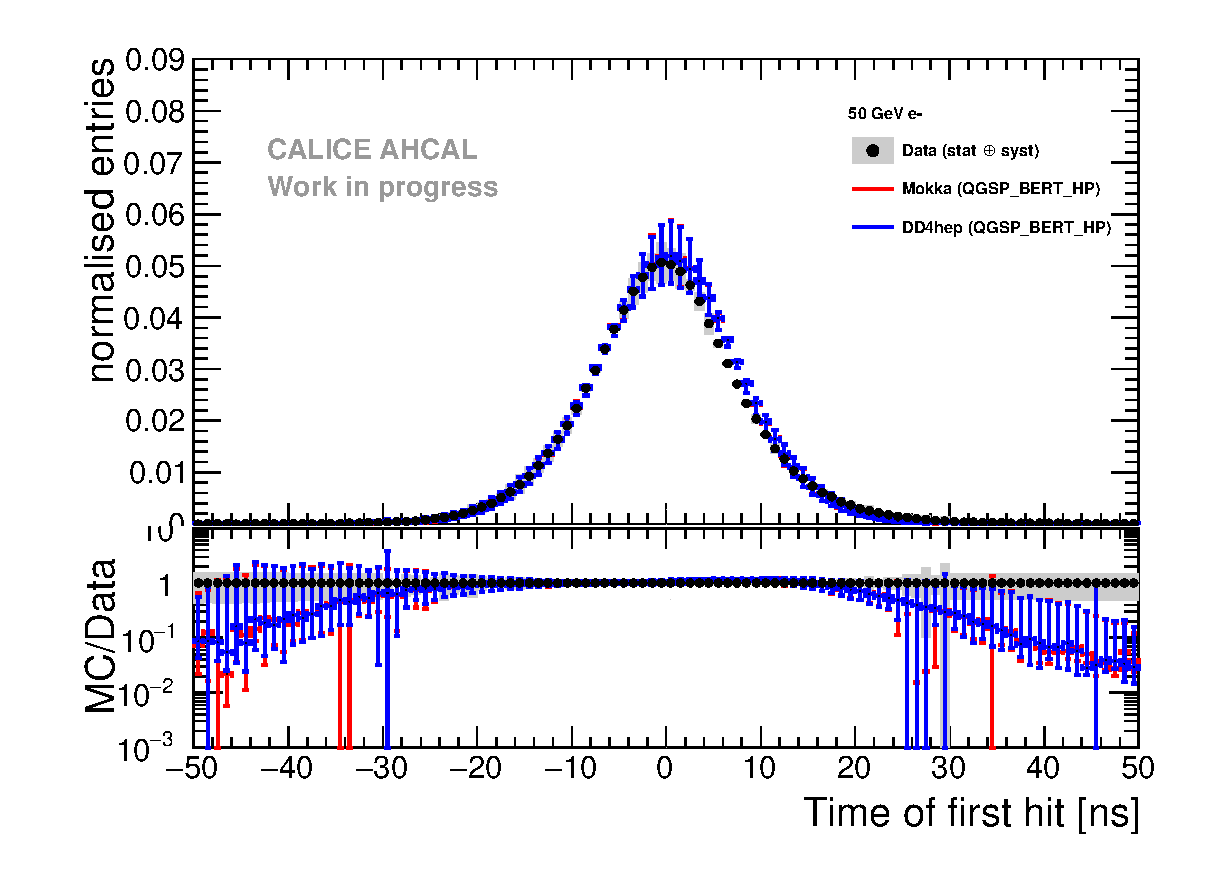
\includegraphics[width=1\textwidth]{../Thesis_Plots/Timing/Electrons/Plots/Comparison_SimData_Electrons50GeV.eps}
    \caption{50 GeV.}\label{fig:elec_sim_data_50GeV}
  \end{subfigure}
  \caption{Comparison between electron data and MC for all energies of the time of first hit. The grey area represents the statistical and systematical error of the data. Error bars in simulation are obtained by varying the cross-talk parameter and with the uncertainty from the number of hits parametrization.} \label{fig:sim_data_elec_add}
\end{figure}

\begin{figure}[htbp!]
  \begin{subfigure}[t]{0.49\textwidth}
    \centering
    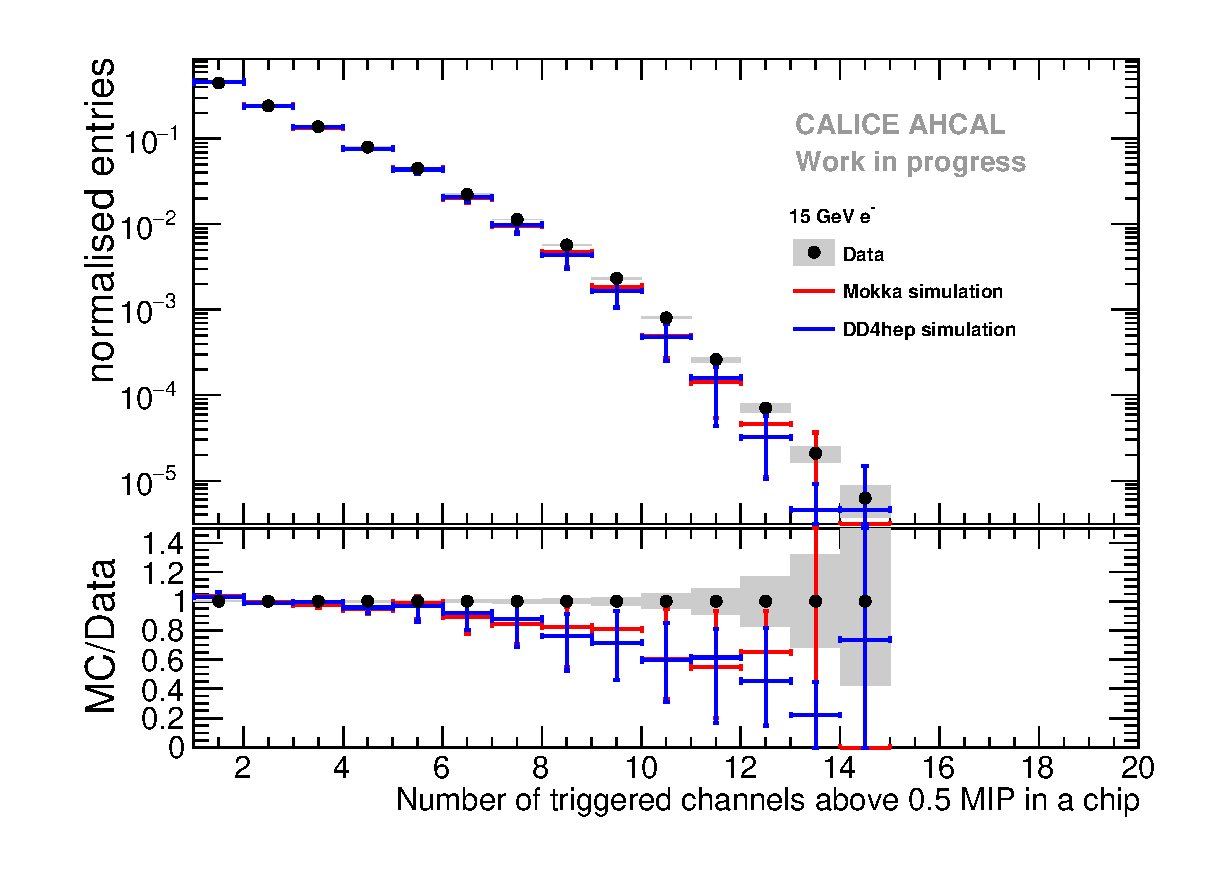
\includegraphics[width=1\textwidth]{../Thesis_Plots/Timing/Electrons/Plots/Comparison_SimData_Electrons_nHits_15GeV.eps}
    \caption{15 GeV.}\label{fig:elec_sim_data_nHits_15GeV}
  \end{subfigure}
  \hfill
  \begin{subfigure}[t]{0.49\textwidth}
    \centering
    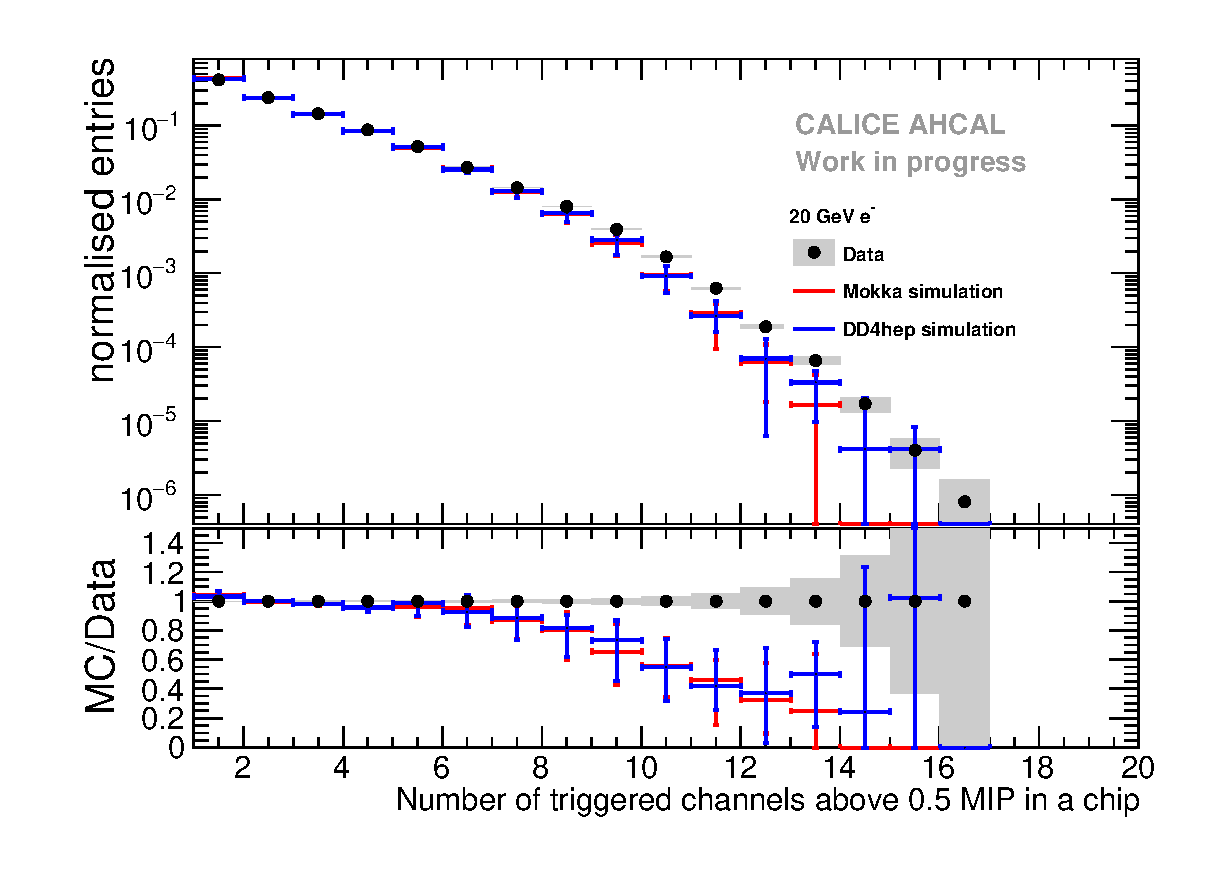
\includegraphics[width=1\textwidth]{../Thesis_Plots/Timing/Electrons/Plots/Comparison_SimData_Electrons_nHits_20GeV.eps}
    \caption{20 GeV.}\label{fig:elec_sim_data_nHits_20GeV}
  \end{subfigure}
  \hfill
  \begin{subfigure}[t]{0.49\textwidth}
    \centering
    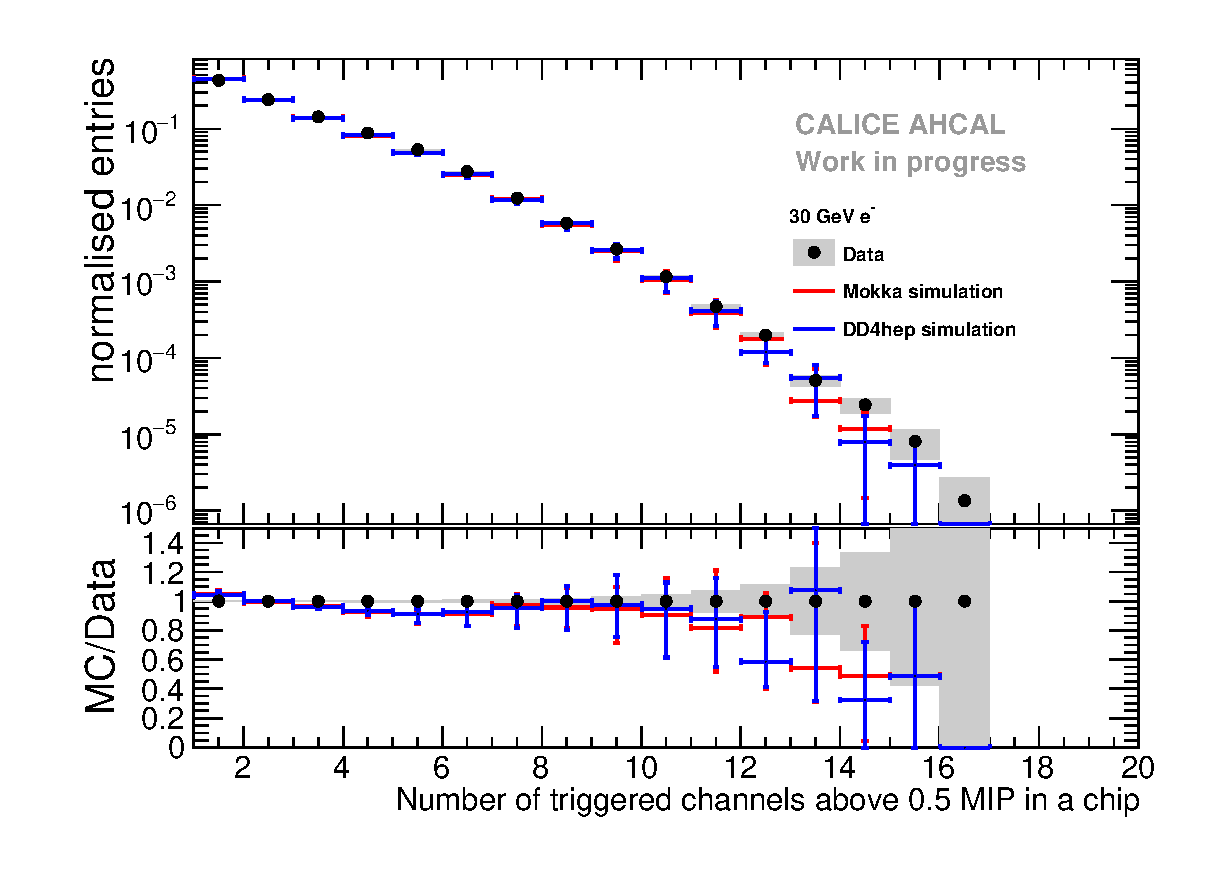
\includegraphics[width=1\textwidth]{../Thesis_Plots/Timing/Electrons/Plots/Comparison_SimData_Electrons_nHits_30GeV.eps}
    \caption{30 GeV.}\label{fig:elec_sim_data_nHits_30GeV}
  \end{subfigure}
  \hfill
  \begin{subfigure}[t]{0.49\textwidth}
    \centering
    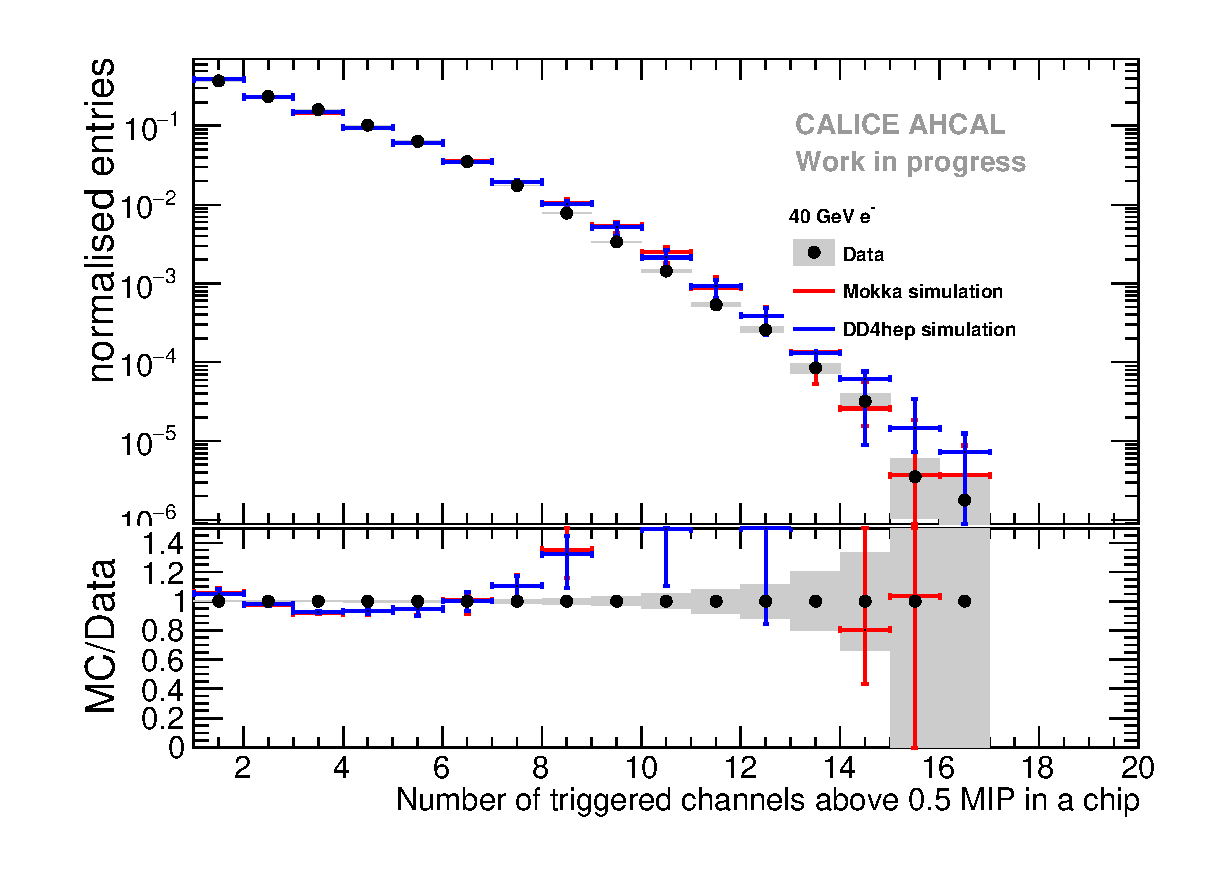
\includegraphics[width=1\textwidth]{../Thesis_Plots/Timing/Electrons/Plots/Comparison_SimData_Electrons_nHits_40GeV.eps}
    \caption{40 GeV.}\label{fig:elec_sim_data_nHits_40GeV}
  \end{subfigure}
  \hfill
  \begin{subfigure}[t]{0.49\textwidth}
    \centering
    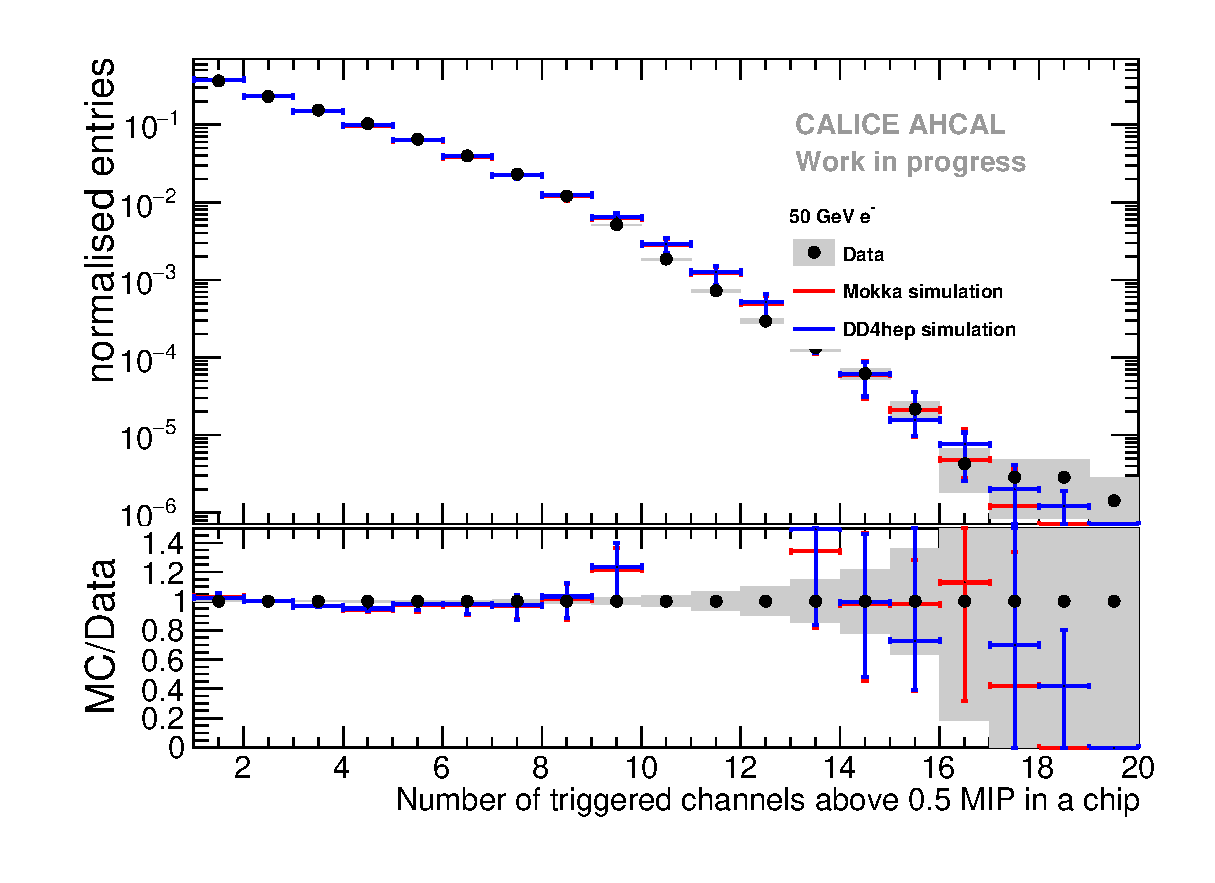
\includegraphics[width=1\textwidth]{../Thesis_Plots/Timing/Electrons/Plots/Comparison_SimData_Electrons_nHits_50GeV.eps}
    \caption{50 GeV.}\label{fig:elec_sim_data_nHits_50GeV}
  \end{subfigure}
  \caption{Comparison between electron data and MC for all energies of the number of triggered channels per chip. The grey area represents the statistical error of the data. Error bars in simulation are obtained by varying the cross-talk parameter between 10\% and 18\%.}
  \label{fig:sim_data_elec_nHits}
\end{figure}

%%%%%%%%%%%%%%%%%%%%%%%%%%%%% Time distribution %%%%%%%%%%%%%%%%%%%%%%%%%%%%%%%%%%%%%%%%%%%%%%%%%%%%%%%%%%%%%%%

\begin{figure}[htbp!]
  \begin{subfigure}[t]{0.49\textwidth}
    \centering
    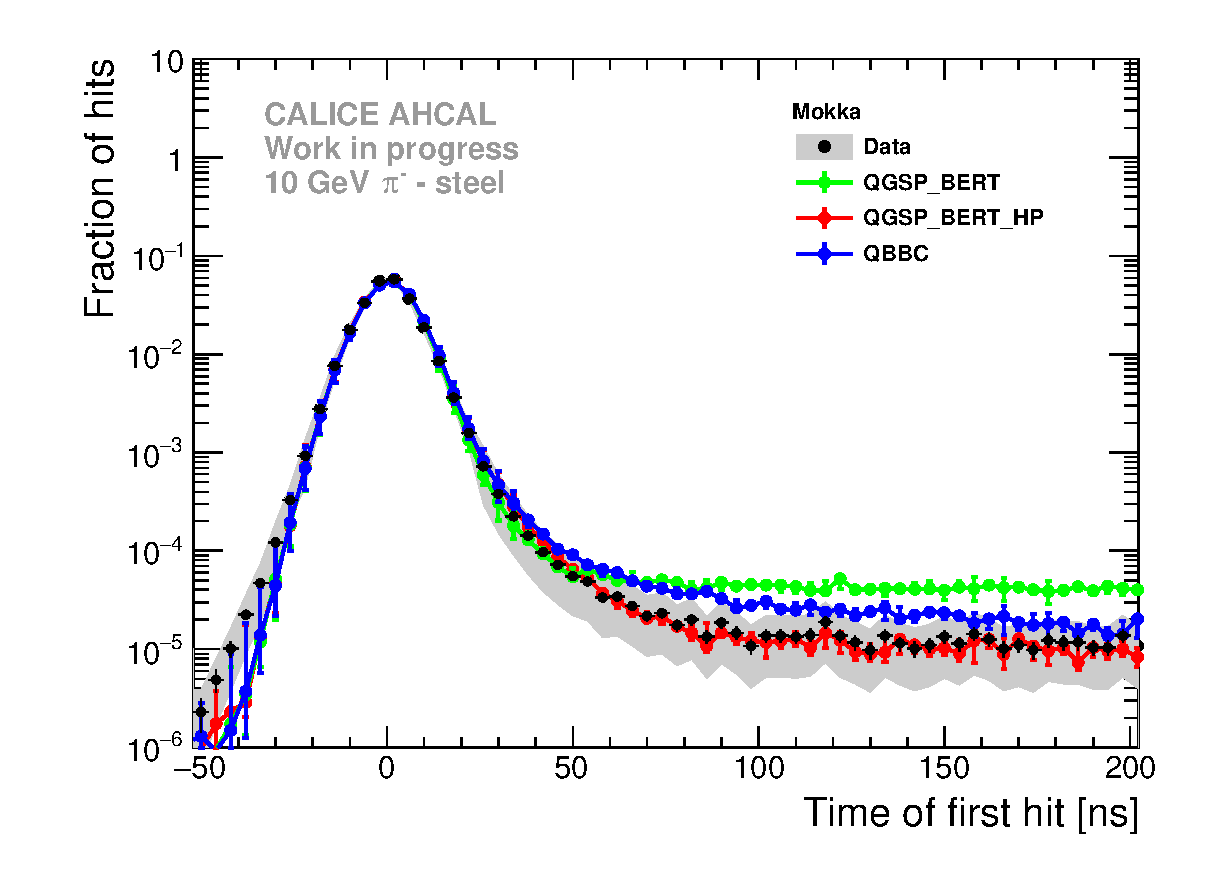
\includegraphics[width=1\textwidth]{../Thesis_Plots/Timing/Pions/Plots/ComparisonToSim/Comparison_SimData_Pion10GeV_LateClusters.eps}
    \caption{10 GeV.} \label{fig:dNdt_SimData_10GeV}
  \end{subfigure}
  \hfill
  \begin{subfigure}[t]{0.49\textwidth}
    \centering
    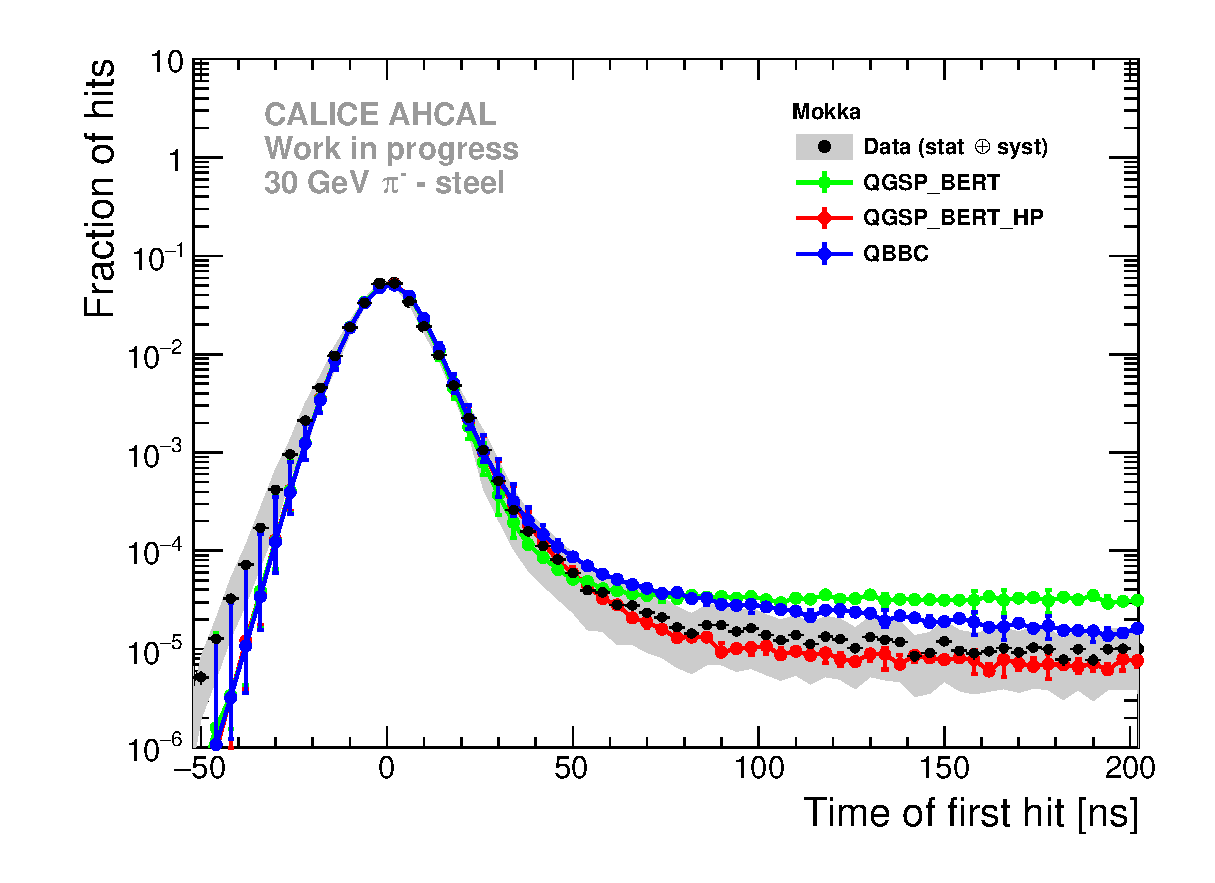
\includegraphics[width=1\textwidth]{../Thesis_Plots/Timing/Pions/Plots/ComparisonToSim/Comparison_SimData_Pion30GeV_LateClusters.eps}
    \caption{30 GeV.}\label{fig:dNdt_SimData_30GeV}
  \end{subfigure}
  \hfill
  \begin{subfigure}[t]{0.49\textwidth}
    \centering
    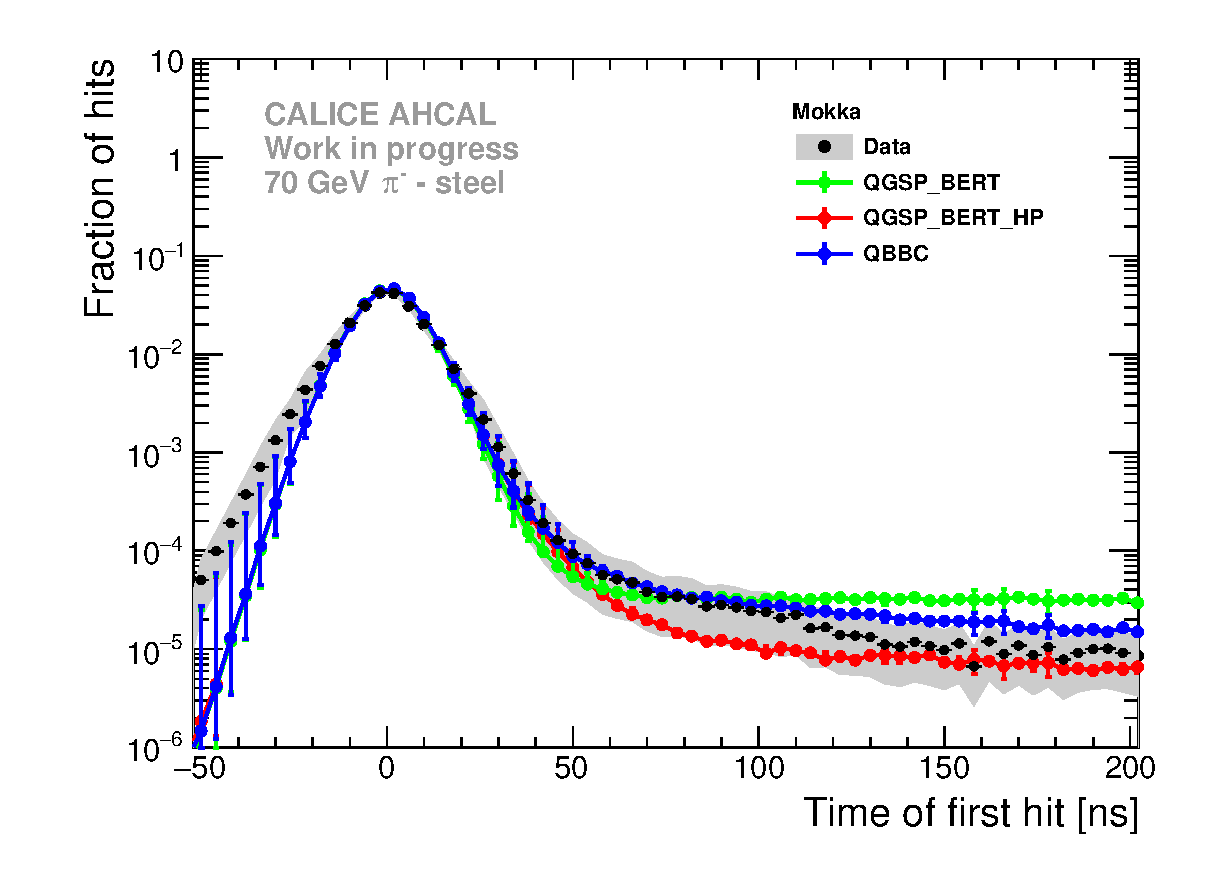
\includegraphics[width=1\textwidth]{../Thesis_Plots/Timing/Pions/Plots/ComparisonToSim/Comparison_SimData_Pion70GeV_LateClusters.eps}
    \caption{70 GeV.} \label{fig:dNdt_SimData_70GeV}
  \end{subfigure}
  \hfill
  \begin{subfigure}[t]{0.49\textwidth}
    \centering
    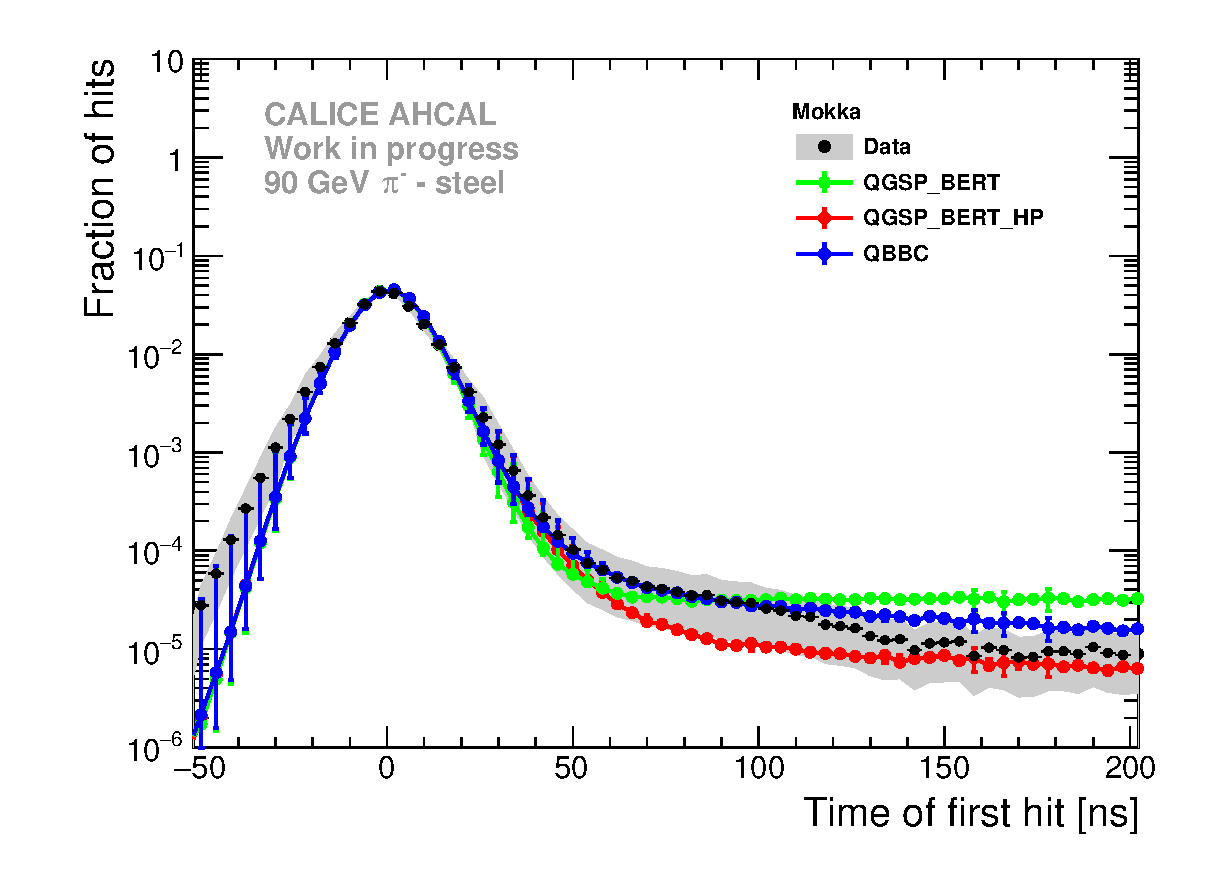
\includegraphics[width=1\textwidth]{../Thesis_Plots/Timing/Pions/Plots/ComparisonToSim/Comparison_SimData_Pion90GeV_LateClusters.eps}
    \caption{90 GeV.} \label{fig:dNdt_SimData_90GeV}
  \end{subfigure}
  \caption{Comparison between data and the \mokka simulation for pions between 10 and 90 GeV of the time of first hit. The grey box represents the statistic and systematic uncertainty of the data. The error bars are the uncertainty on the \mokka simulation obtained by varying the cross-talk parameter and the uncertainty on the time smearing.}
\end{figure}

\begin{figure}[htbp!]
  \begin{subfigure}[t]{0.49\textwidth}
    \centering
    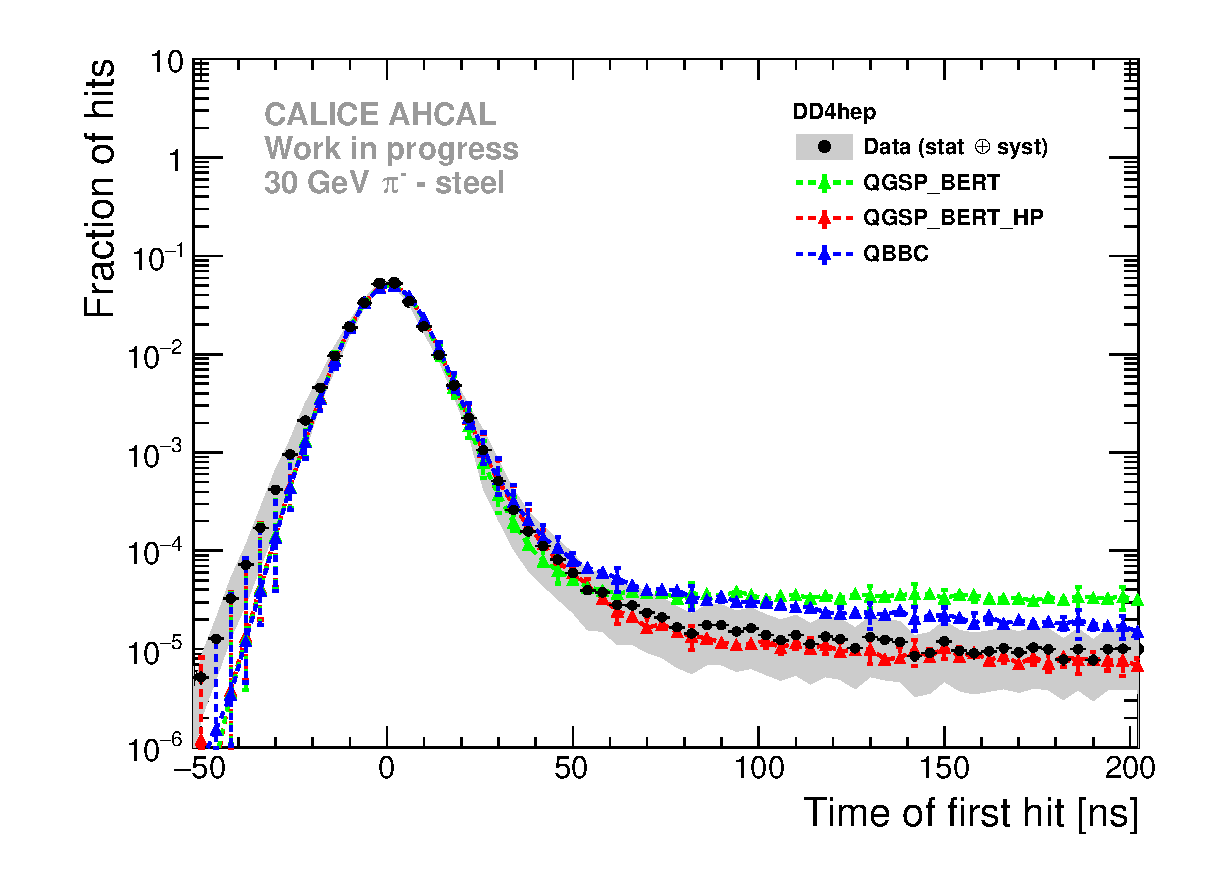
\includegraphics[width=1\textwidth]{../Thesis_Plots/Timing/Pions/Plots/ComparisonToSim/Comparison_SimData_Pion30GeV_LateClusters_DD4hep.eps}
    \caption{30 GeV.}\label{fig:dNdt_SimData_30GeV_DD4hep}
  \end{subfigure}
  \hfill
  \begin{subfigure}[t]{0.49\textwidth}
    \centering
    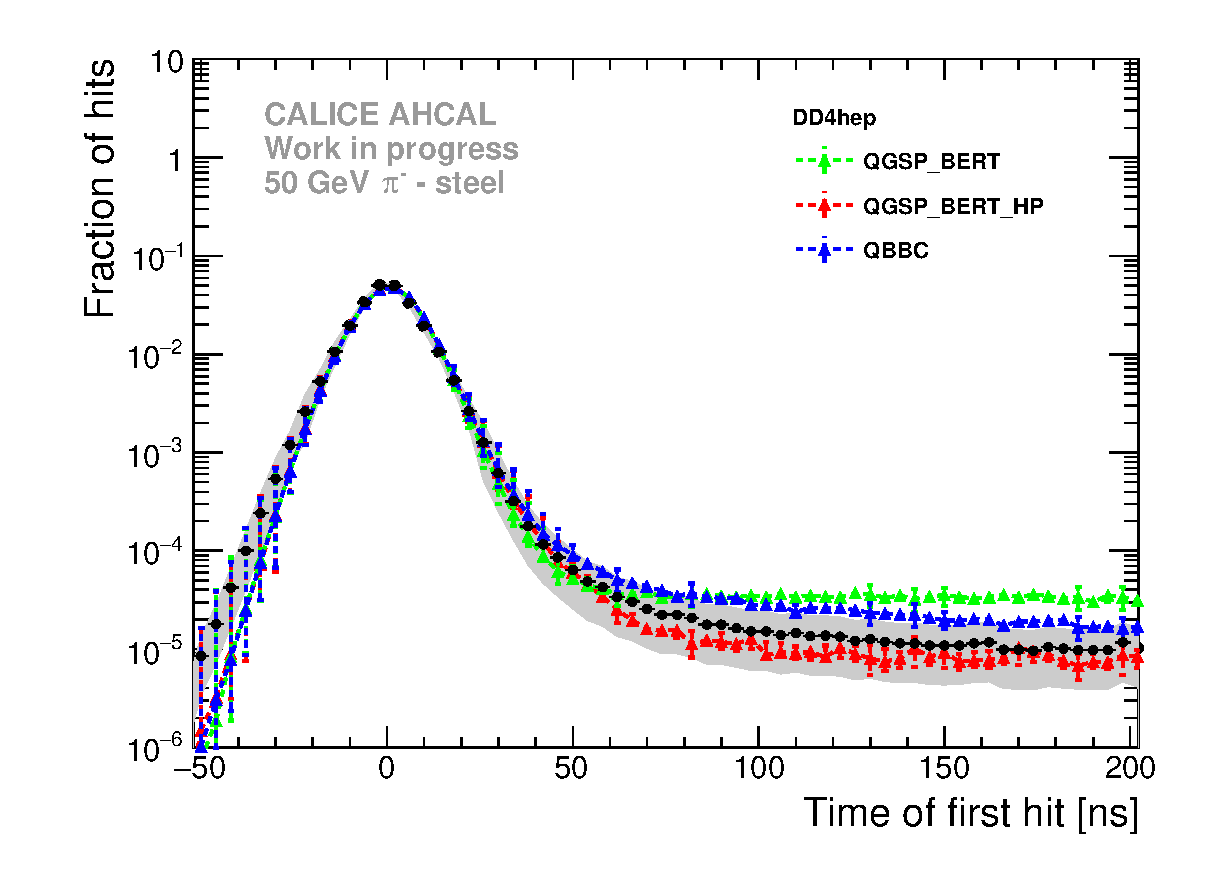
\includegraphics[width=1\textwidth]{../Thesis_Plots/Timing/Pions/Plots/ComparisonToSim/Comparison_SimData_Pion50GeV_LateClusters_DD4hep.eps}
    \caption{50 GeV.} \label{fig:dNdt_SimData_50GeV_DD4hep}
  \end{subfigure}
  \hfill
  \begin{subfigure}[t]{0.49\textwidth}
    \centering
    \includegraphics[width=1\textwidth]{../Thesis_Plots/Timing/Pions/Plots/ComparisonToSim/Comparison_SimData_Pion70GeV_LateClusters_DD4hep.eps}
    \caption{70 GeV.} \label{fig:dNdt_SimData_70GeV_DD4hep}
  \end{subfigure}
  \hfill
  \begin{subfigure}[t]{0.49\textwidth}
    \centering
    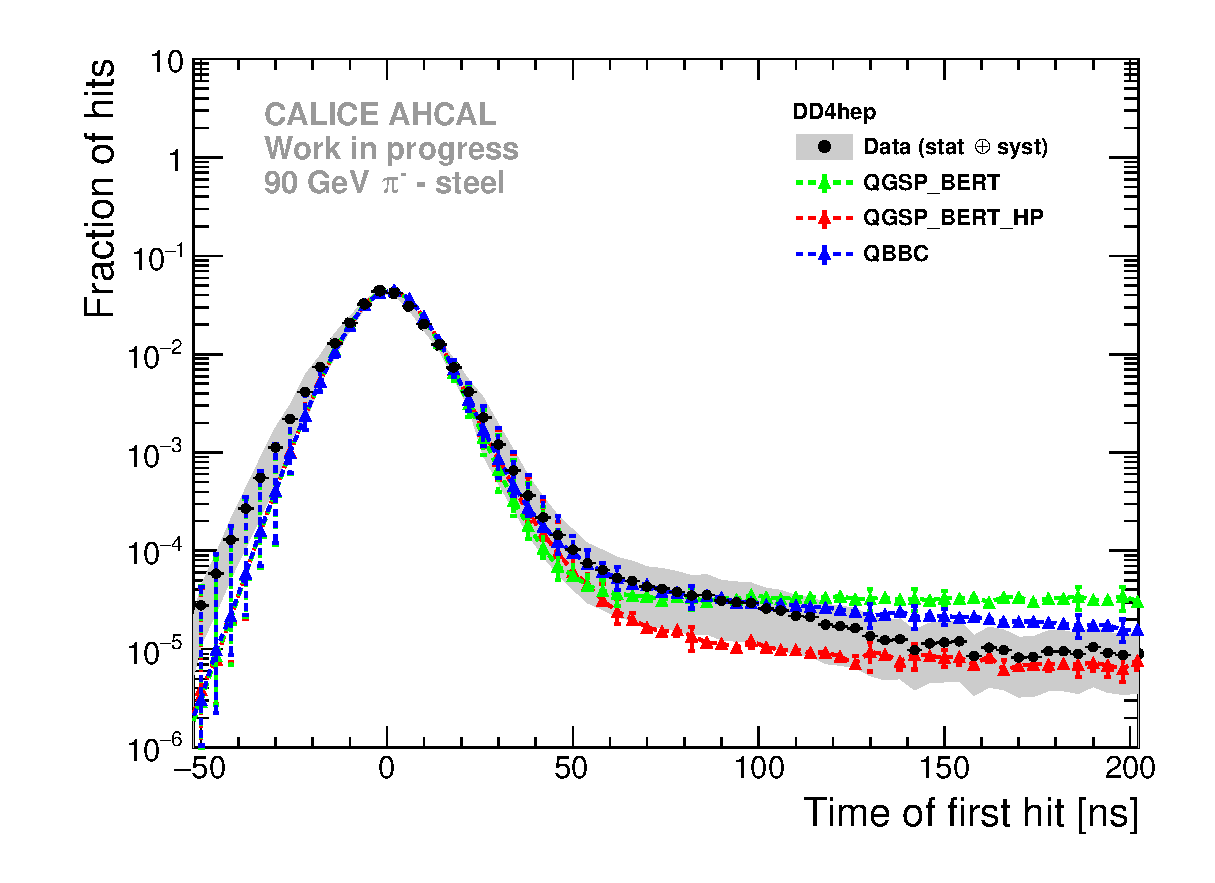
\includegraphics[width=1\textwidth]{../Thesis_Plots/Timing/Pions/Plots/ComparisonToSim/Comparison_SimData_Pion90GeV_LateClusters_DD4hep.eps}
    \caption{90 GeV.} \label{fig:dNdt_SimData_90GeV_DD4hep}
  \end{subfigure}
  \caption{Comparison between data and the \ddhep simulation for pions between 30 and 90 GeV of the time of first hit. The grey box represents the statistic and systematic uncertainty of the data. The error bars are the uncertainty on the \ddhep simulation obtained by varying the cross-talk parameter and the uncertainty on the time smearing.}
\end{figure}


%%%%%%%%%%%%%%%%%%%%%%%%%%%%% Energy %%%%%%%%%%%%%%%%%%%%%%%%%%%%%%%%%%%%%%%%%%%%%%%%%%%%%%%%%%%%%%%

\begin{figure}[htbp!]
  \begin{subfigure}[t]{0.49\textwidth}
    \centering
    \includegraphics[width=1\textwidth]{../Thesis_Plots/Timing/Pions/Plots/ComparisonToSim/Time_Energy_30GeV_Mokka.eps}
    \caption{30 GeV.}\label{fig:Energy_SimData_30GeV}
  \end{subfigure}
  \hfill
  \begin{subfigure}[t]{0.49\textwidth}
    \centering
    \includegraphics[width=1\textwidth]{../Thesis_Plots/Timing/Pions/Plots/ComparisonToSim/Time_Energy_50GeV_Mokka.eps}
    \caption{50 GeV.} \label{fig:Energy_SimData_50GeV}
  \end{subfigure}
  \hfill
  \begin{subfigure}[t]{0.49\textwidth}
    \centering
    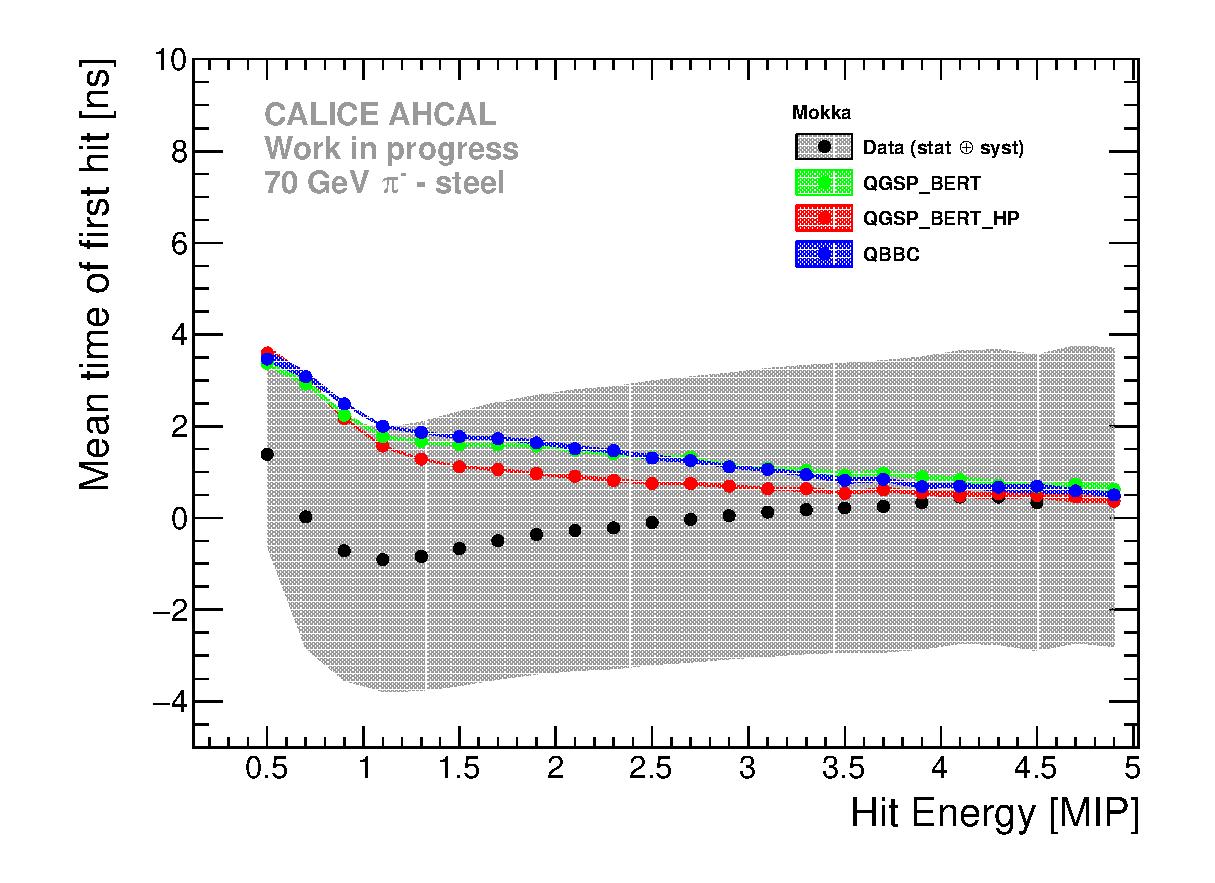
\includegraphics[width=1\textwidth]{../Thesis_Plots/Timing/Pions/Plots/ComparisonToSim/Time_Energy_70GeV_Mokka.eps}
    \caption{70 GeV.} \label{fig:Energy_SimData_70GeV}
  \end{subfigure}
  \caption{Comparison between the \mokka simulation and data of the time of first hit as a function of the hit energy for pion beams between 30 GeV and 70 GeV. The grey and color bands shows the systematics.}
\end{figure}

\begin{figure}[htbp!]
  \begin{subfigure}[t]{0.49\textwidth}
    \centering
    \includegraphics[width=1\textwidth]{../Thesis_Plots/Timing/Pions/Plots/ComparisonToSim/Time_Energy_10GeV_DD4hep.eps}
    \caption{10 GeV.}\label{fig:Energy_SimData_10GeV_DD4hep}
  \end{subfigure}
  \hfill
  \begin{subfigure}[t]{0.49\textwidth}
    \centering
    \includegraphics[width=1\textwidth]{../Thesis_Plots/Timing/Pions/Plots/ComparisonToSim/Time_Energy_30GeV_DD4hep.eps}
    \caption{30 GeV.}\label{fig:Energy_SimData_30GeV_DD4hep}
  \end{subfigure}
  \hfill
  \begin{subfigure}[t]{0.49\textwidth}
    \centering
    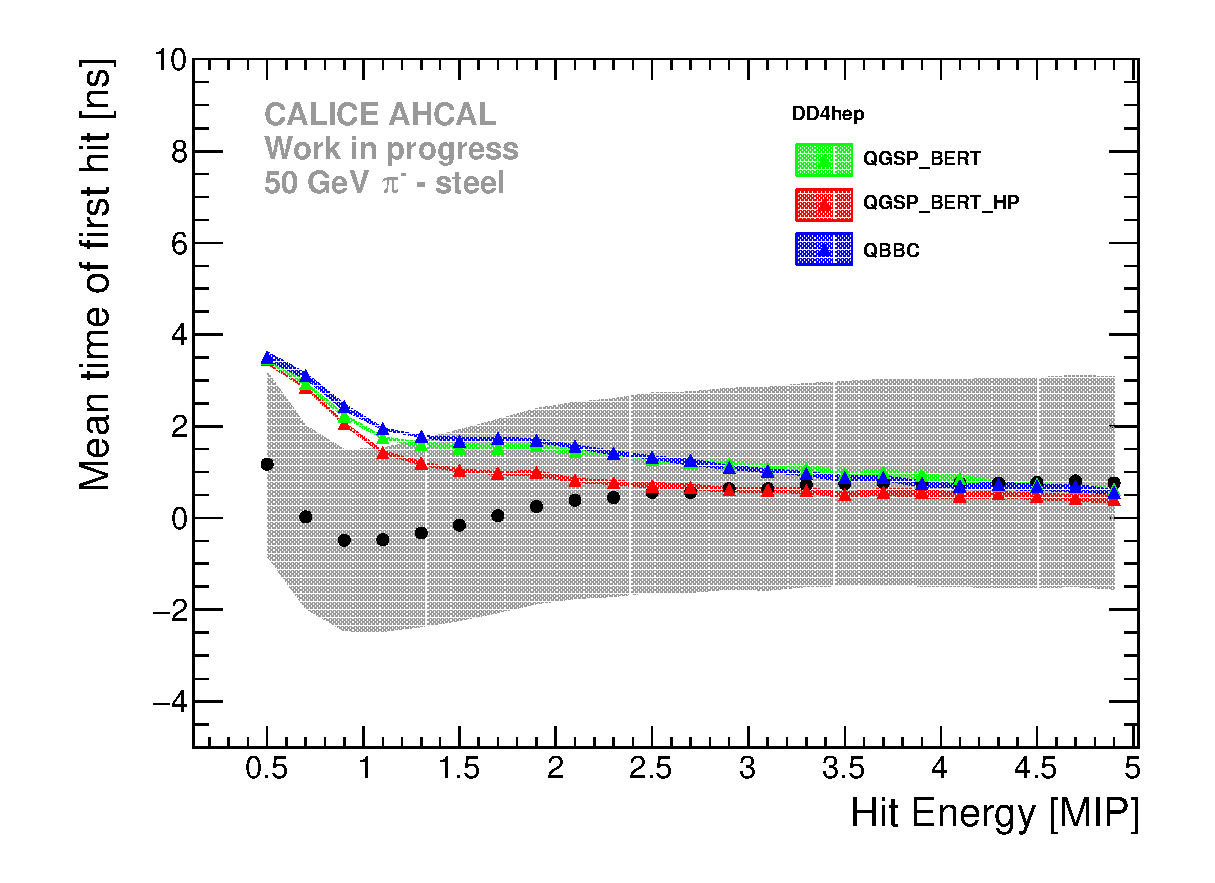
\includegraphics[width=1\textwidth]{../Thesis_Plots/Timing/Pions/Plots/ComparisonToSim/Time_Energy_50GeV_DD4hep.eps}
    \caption{50 GeV.} \label{fig:Energy_SimData_50GeV_DD4hep}
  \end{subfigure}
  \hfill
  \begin{subfigure}[t]{0.49\textwidth}
    \centering
    \includegraphics[width=1\textwidth]{../Thesis_Plots/Timing/Pions/Plots/ComparisonToSim/Time_Energy_70GeV_DD4hep.eps}
    \caption{70 GeV.} \label{fig:Energy_SimData_70GeV_DD4hep}
  \end{subfigure}
  \hfill
  \begin{subfigure}[t]{0.49\textwidth}
    \centering
    \includegraphics[width=1\textwidth]{../Thesis_Plots/Timing/Pions/Plots/ComparisonToSim/Time_Energy_90GeV_DD4hep.eps}
    \caption{90 GeV.} \label{fig:Energy_SimData_90GeV_DD4hep}
  \end{subfigure}
  \caption{Comparison between the \ddhep simulation and data of the time of first hit as a function of the hit energy for pion beams between 10 GeV and 90 GeV. The grey and color bands shows the systematics.}
\end{figure}

%%%%%%%%%%%%%%%%%%%%%%%%%%%%% Radius %%%%%%%%%%%%%%%%%%%%%%%%%%%%%%%%%%%%%%%%%%%%%%%%%%%%%%%%%%%%%%%

\begin{figure}[htbp!]
  \begin{subfigure}[t]{0.49\textwidth}
    \centering
    \includegraphics[width=1\textwidth]{../Thesis_Plots/Timing/Pions/Plots/ComparisonToSim/Time_Radius_10GeV_SSF_Mokka.eps}
    \caption{10 GeV.} \label{fig:Radius_SSF_SimData_10GeV}
  \end{subfigure}
  \hfill
  \begin{subfigure}[t]{0.49\textwidth}
    \centering
    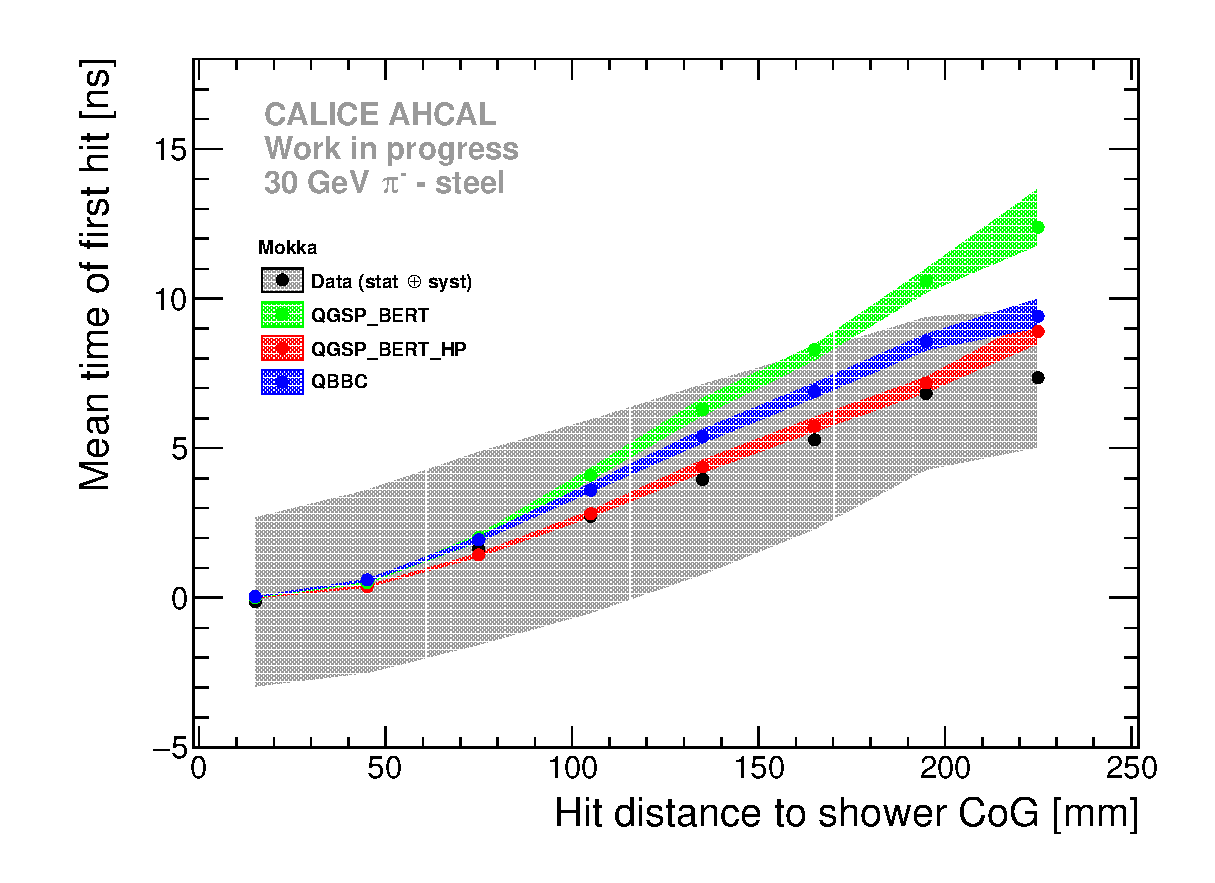
\includegraphics[width=1\textwidth]{../Thesis_Plots/Timing/Pions/Plots/ComparisonToSim/Time_Radius_30GeV_SSF_Mokka.eps}
    \caption{50 GeV.} \label{fig:Radius_SSF_SimData_30GeV}
  \end{subfigure}
  \hfill
  \begin{subfigure}[t]{0.49\textwidth}
    \centering
    \includegraphics[width=1\textwidth]{../Thesis_Plots/Timing/Pions/Plots/ComparisonToSim/Time_Radius_70GeV_SSF_Mokka.eps}
    \caption{70 GeV.} \label{fig:Radius_SSF_SimData_70GeV}
  \end{subfigure}
  \hfill
  \begin{subfigure}[t]{0.49\textwidth}
    \centering
    \includegraphics[width=1\textwidth]{../Thesis_Plots/Timing/Pions/Plots/ComparisonToSim/Time_Radius_90GeV_SSF_Mokka.eps}
    \caption{90 GeV.} \label{fig:Radius_SSF_SimData_90GeV}
  \end{subfigure}
  \caption{Comparison of the time of first hit as a function of the hit distance to the shower axis in data and the \mokka simulation for pion beam energies between 10 GeV and 90 GeV for modules 3 to 10. The grey and color bands shows the systematics.}
\end{figure}

\begin{figure}[htbp!]
  \begin{subfigure}[t]{0.49\textwidth}
    \centering
    \includegraphics[width=1\textwidth]{../Thesis_Plots/Timing/Pions/Plots/ComparisonToSim/Time_Radius_10GeV_SSF_DD4hep.eps}
    \caption{10 GeV.} \label{fig:Radius_SSF_SimData_10GeV_DD4hep}
  \end{subfigure}
  \hfill
  \begin{subfigure}[t]{0.49\textwidth}
    \centering
    \includegraphics[width=1\textwidth]{../Thesis_Plots/Timing/Pions/Plots/ComparisonToSim/Time_Radius_30GeV_SSF_DD4hep.eps}
    \caption{30 GeV.} \label{fig:Radius_SSF_SimData_30GeV_DD4hep}
  \end{subfigure}
  \hfill
  \begin{subfigure}[t]{0.49\textwidth}
    \centering
    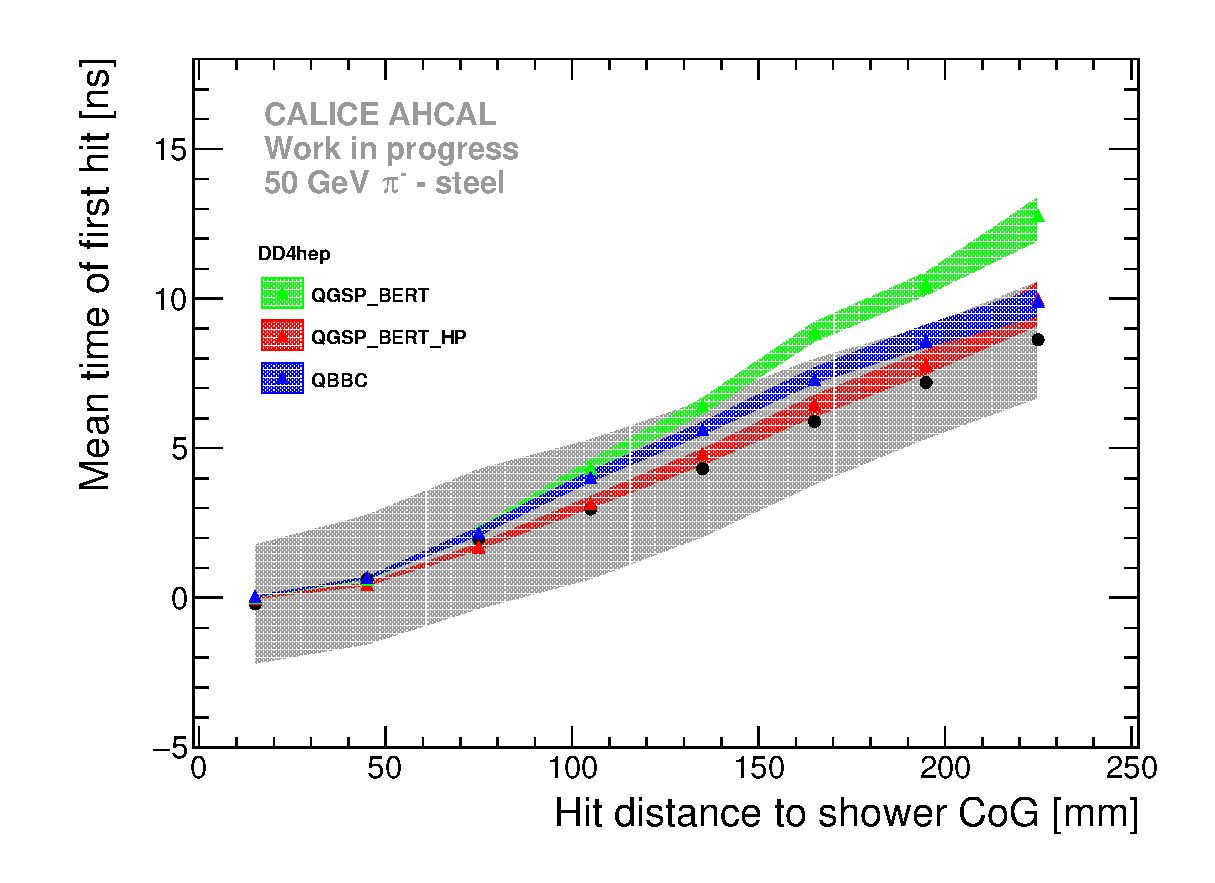
\includegraphics[width=1\textwidth]{../Thesis_Plots/Timing/Pions/Plots/ComparisonToSim/Time_Radius_50GeV_SSF_DD4hep.eps}
    \caption{50 GeV.} \label{fig:Radius_SSF_SimData_50GeV_DD4hep}
  \end{subfigure}
  \hfill
  \begin{subfigure}[t]{0.49\textwidth}
    \centering
    \includegraphics[width=1\textwidth]{../Thesis_Plots/Timing/Pions/Plots/ComparisonToSim/Time_Radius_70GeV_SSF_DD4hep.eps}
    \caption{70 GeV.} \label{fig:Radius_SSF_SimData_70GeV_DD4hep}
  \end{subfigure}
  \hfill
  \begin{subfigure}[t]{0.49\textwidth}
    \centering
    \includegraphics[width=1\textwidth]{../Thesis_Plots/Timing/Pions/Plots/ComparisonToSim/Time_Radius_90GeV_SSF_DD4hep.eps}
    \caption{90 GeV.} \label{fig:Radius_SSF_SimData_90GeV_DD4hep}
  \end{subfigure}
  \caption{Comparison of the time of first hit as a function of the hit distance to the shower axis in data and the \ddhep simulation for pion beam energies between 10 GeV and 90 GeV for modules 3 to 10. The grey and color bands shows the systematics.}
\end{figure}

\begin{figure}[htbp!]
  \begin{subfigure}[t]{0.49\textwidth}
    \centering
    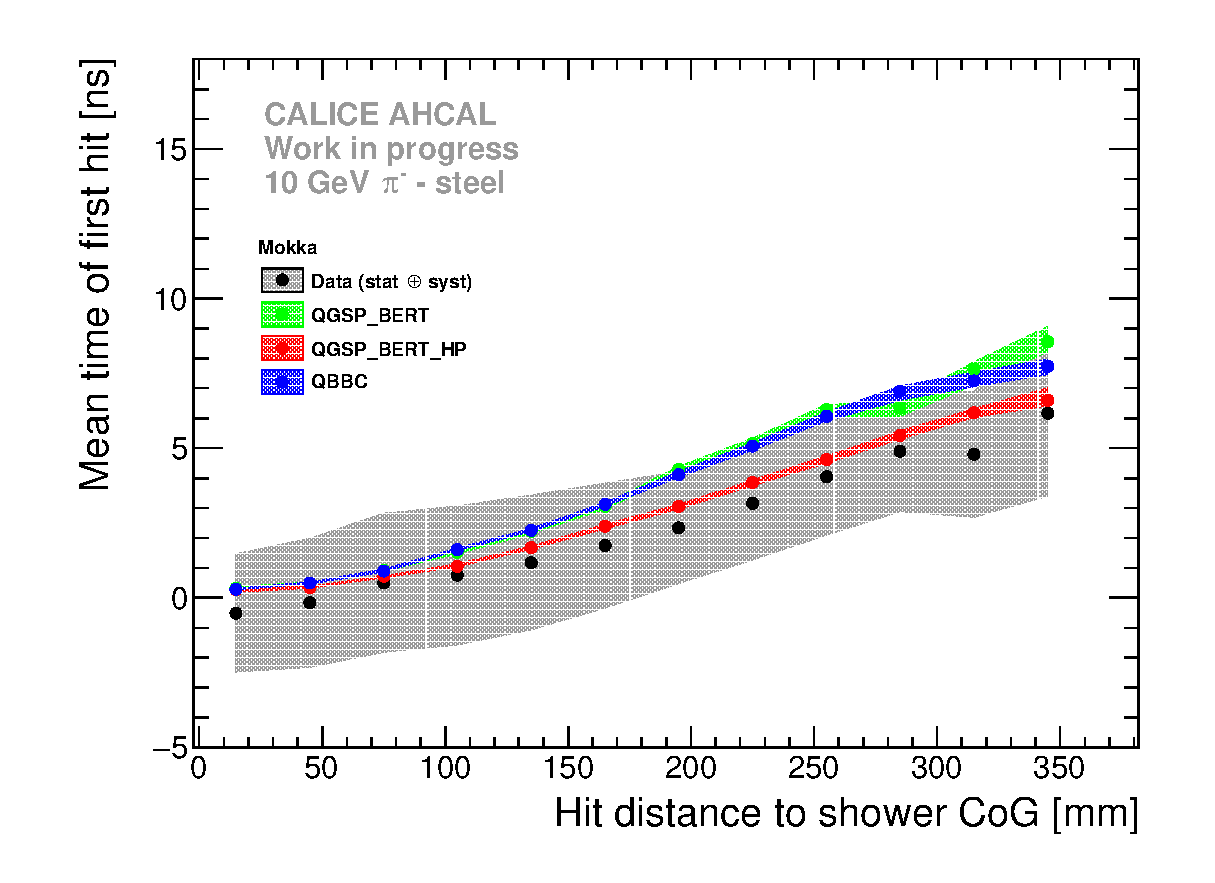
\includegraphics[width=1\textwidth]{../Thesis_Plots/Timing/Pions/Plots/ComparisonToSim/Time_Radius_10GeV_BL_Mokka.eps}
    \caption{10 GeV.} \label{fig:Radius_BL_SimData_10GeV}
  \end{subfigure}
  \hfill
  \begin{subfigure}[t]{0.49\textwidth}
    \centering
    \includegraphics[width=1\textwidth]{../Thesis_Plots/Timing/Pions/Plots/ComparisonToSim/Time_Radius_30GeV_BL_Mokka.eps}
    \caption{30 GeV.} \label{fig:Radius_BL_SimData_30GeV}
  \end{subfigure}
  \hfill
  \begin{subfigure}[t]{0.49\textwidth}
    \centering
    \includegraphics[width=1\textwidth]{../Thesis_Plots/Timing/Pions/Plots/ComparisonToSim/Time_Radius_70GeV_BL_Mokka.eps}
    \caption{70 GeV.} \label{fig:Radius_BL_SimData_70GeV}
  \end{subfigure}
  \hfill
  \begin{subfigure}[t]{0.49\textwidth}
    \centering
    \includegraphics[width=1\textwidth]{../Thesis_Plots/Timing/Pions/Plots/ComparisonToSim/Time_Radius_90GeV_BL_Mokka.eps}
    \caption{90 GeV.} \label{fig:Radius_BL_SimData_90GeV}
  \end{subfigure}
  \caption{Comparison of the time of first hit as a function of the hit distance to the shower axis in data and the \mokka simulation for pion beam energies between 10 GeV and 90 GeV for modules 11 to 14. The grey and color bands shows the systematics.}
\end{figure}

\begin{figure}[htbp!]
  \begin{subfigure}[t]{0.49\textwidth}
    \centering
    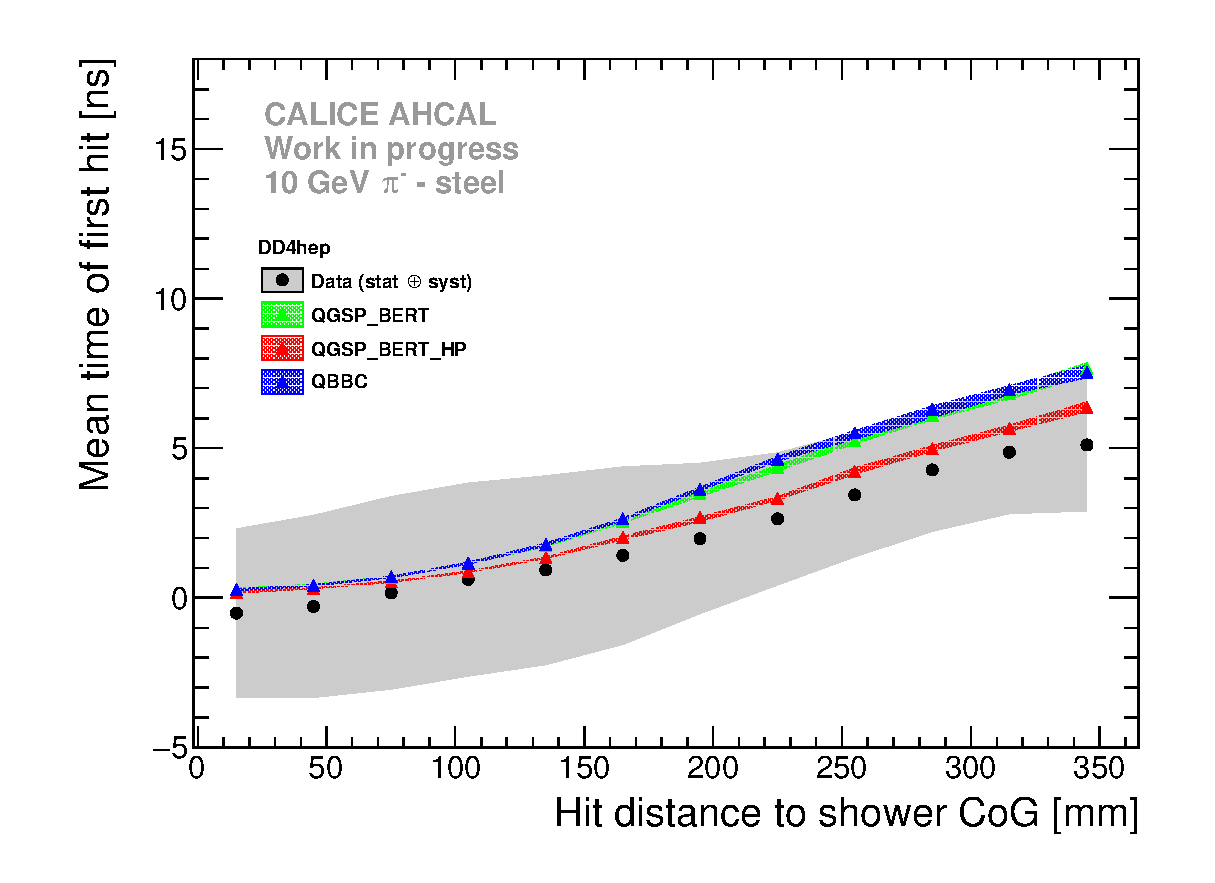
\includegraphics[width=1\textwidth]{../Thesis_Plots/Timing/Pions/Plots/ComparisonToSim/Time_Radius_10GeV_BL_DD4hep.eps}
    \caption{10 GeV.}\label{fig:Radius_BL_SimData_10GeV_DD4hep}
  \end{subfigure}
  \hfill
  \begin{subfigure}[t]{0.49\textwidth}
    \centering
    \includegraphics[width=1\textwidth]{../Thesis_Plots/Timing/Pions/Plots/ComparisonToSim/Time_Radius_30GeV_BL_DD4hep.eps}
    \caption{30 GeV.} \label{fig:Radius_BL_SimData_30GeV_DD4hep}
  \end{subfigure}
  \hfill
  \begin{subfigure}[t]{0.49\textwidth}
    \centering
    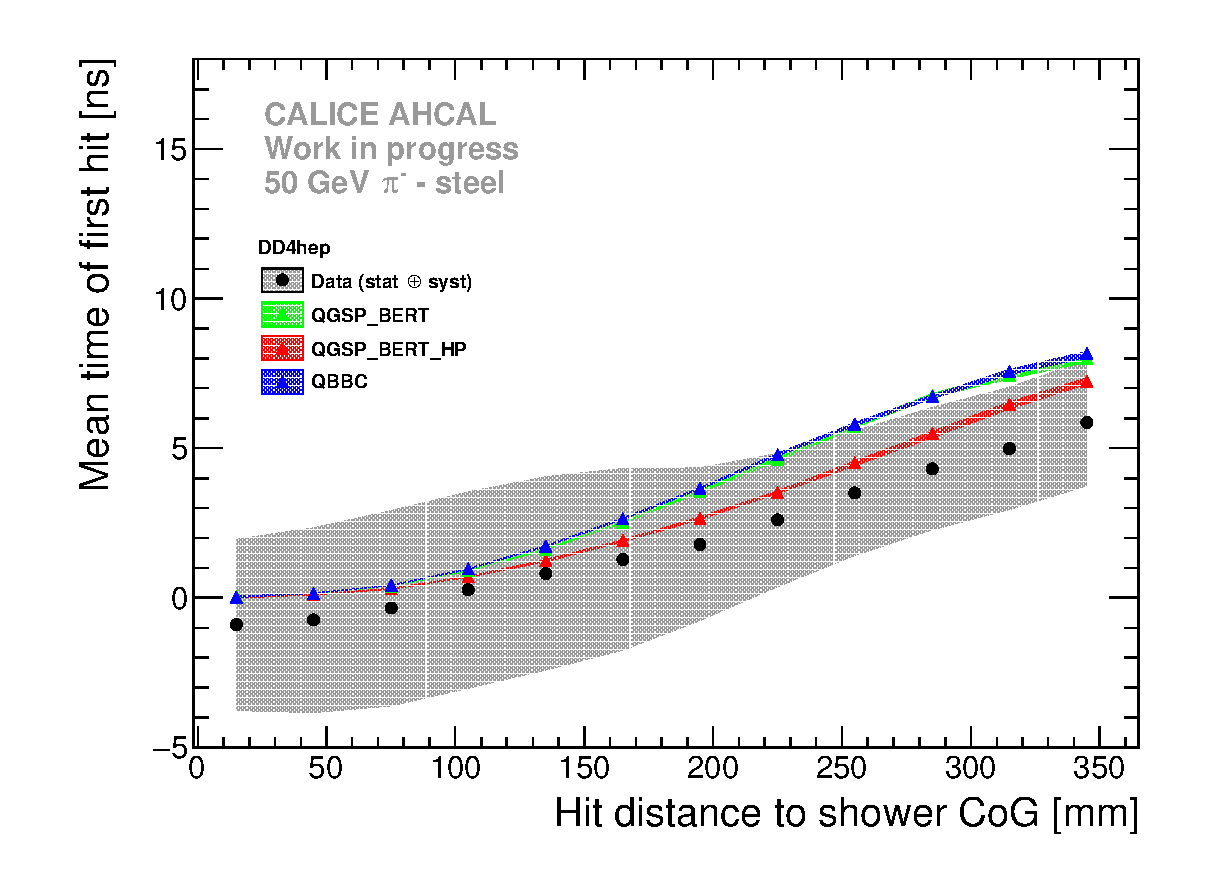
\includegraphics[width=1\textwidth]{../Thesis_Plots/Timing/Pions/Plots/ComparisonToSim/Time_Radius_50GeV_BL_DD4hep.eps}
    \caption{50 GeV.} \label{fig:Radius_BL_SimData_50GeV_DD4hep}
  \end{subfigure}
  \hfill
  \begin{subfigure}[t]{0.49\textwidth}
    \centering
    \includegraphics[width=1\textwidth]{../Thesis_Plots/Timing/Pions/Plots/ComparisonToSim/Time_Radius_70GeV_BL_DD4hep.eps}
    \caption{70 GeV.} \label{fig:Radius_BL_SimData_70GeV_DD4hep}
  \end{subfigure}
  \hfill
  \begin{subfigure}[t]{0.49\textwidth}
    \centering
    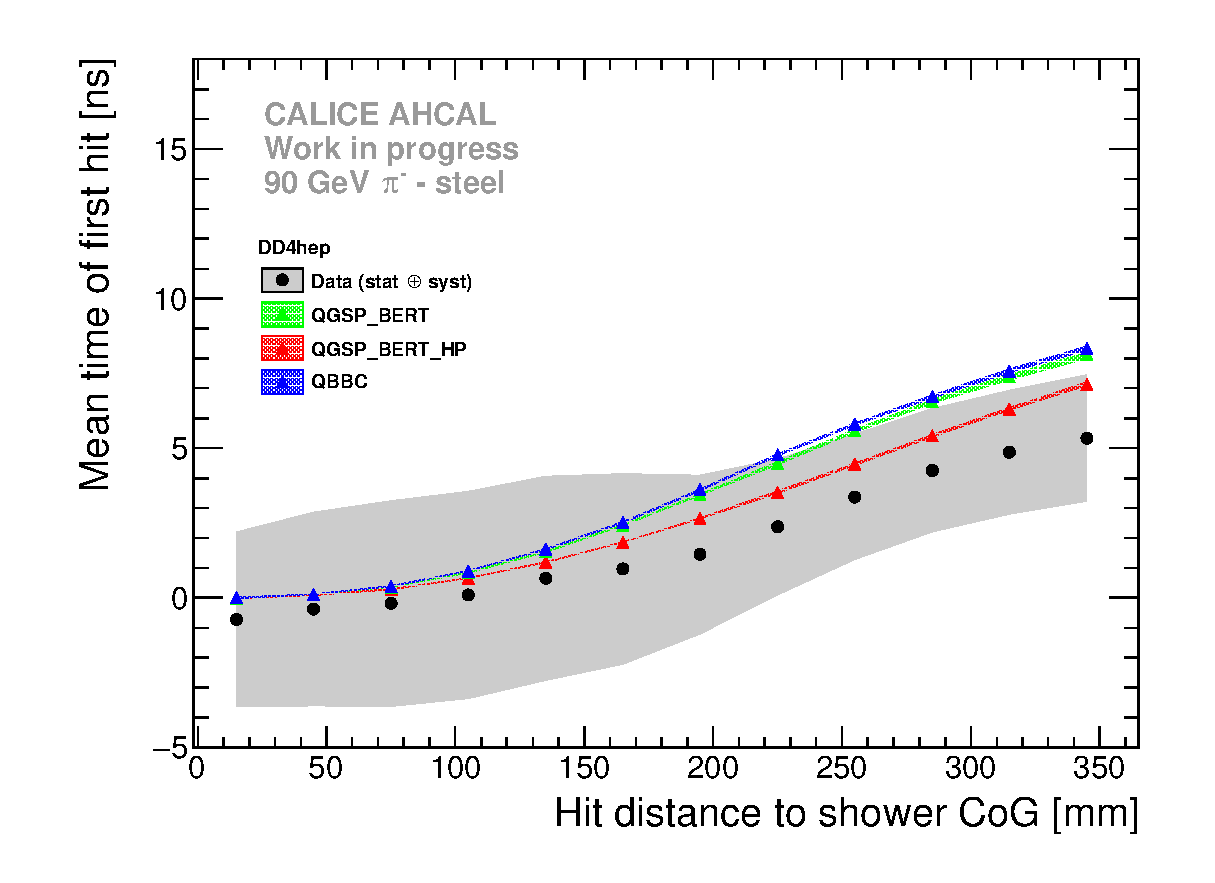
\includegraphics[width=1\textwidth]{../Thesis_Plots/Timing/Pions/Plots/ComparisonToSim/Time_Radius_90GeV_BL_DD4hep.eps}
    \caption{90 GeV.} \label{fig:Radius_BL_SimData_90GeV_DD4hep}
  \end{subfigure}
  \caption{Comparison of the time of first hit as a function of the hit distance to the shower axis in data and the \ddhep simulation for pion beam energies between 10 GeV and 90 GeV for modules 11 to 14. The grey and color bands shows the systematics.}
  \label{fig:Radius_BL_SimData_Comparison_DD4hep}
\end{figure}

%%%%%%%%%%%%%%%%%%%%%%%%%%%%% Depth %%%%%%%%%%%%%%%%%%%%%%%%%%%%%%%%%%%%%%%%%%%%%%%%%%%%%%%%%%%%%%%

\begin{figure}[htbp!]
  \begin{subfigure}[t]{0.49\textwidth}
    \centering
    \includegraphics[width=1\textwidth]{../Thesis_Plots/Timing/Pions/Plots/ComparisonToSim/Time_Depth_10GeV_Mokka.eps}
    \caption{10 GeV.}\label{fig:Depth_SimData_10GeV}
  \end{subfigure}
  \hfill
  \begin{subfigure}[t]{0.49\textwidth}
    \centering
    \includegraphics[width=1\textwidth]{../Thesis_Plots/Timing/Pions/Plots/ComparisonToSim/Time_Depth_30GeV_Mokka.eps}
    \caption{30 GeV.} \label{fig:Depth_SimData_30GeV}
  \end{subfigure}
  \hfill
  \begin{subfigure}[t]{0.49\textwidth}
    \centering
    \includegraphics[width=1\textwidth]{../Thesis_Plots/Timing/Pions/Plots/ComparisonToSim/Time_Depth_50GeV_Mokka.eps}
    \caption{50 GeV.} \label{fig:Depth_SimData_50GeV}
  \end{subfigure}
  \hfill
  \begin{subfigure}[t]{0.49\textwidth}
    \centering
    \includegraphics[width=1\textwidth]{../Thesis_Plots/Timing/Pions/Plots/ComparisonToSim/Time_Depth_70GeV_Mokka.eps}
    \caption{70 GeV.} \label{fig:Depth_SimData_70GeV}
  \end{subfigure}
  \caption{Comparison of the time of first hit as a function of the layer position in data and the \mokka simulation for pion beams between 10 GeV and 70 GeV. The grey and color bands shows the systematics.}
\end{figure}

\begin{figure}[htbp!]
  \begin{subfigure}[t]{0.49\textwidth}
    \centering
    \includegraphics[width=1\textwidth]{../Thesis_Plots/Timing/Pions/Plots/ComparisonToSim/Time_Depth_10GeV_DD4hep.eps}
    \caption{10 GeV.}\label{fig:Depth_SimData_10GeV_DD4hep}
  \end{subfigure}
  \hfill
  \begin{subfigure}[t]{0.49\textwidth}
    \centering
    \includegraphics[width=1\textwidth]{../Thesis_Plots/Timing/Pions/Plots/ComparisonToSim/Time_Depth_30GeV_DD4hep.eps}
    \caption{30 GeV.} \label{fig:Depth_SimData_30GeV_DD4hep}
  \end{subfigure}
  \hfill
  \begin{subfigure}[t]{0.49\textwidth}
    \centering
    \includegraphics[width=1\textwidth]{../Thesis_Plots/Timing/Pions/Plots/ComparisonToSim/Time_Depth_50GeV_DD4hep.eps}
    \caption{50 GeV.} \label{fig:Depth_SimData_50GeV_DD4hep}
  \end{subfigure}
  \hfill
  \begin{subfigure}[t]{0.49\textwidth}
    \centering
    \includegraphics[width=1\textwidth]{../Thesis_Plots/Timing/Pions/Plots/ComparisonToSim/Time_Depth_70GeV_DD4hep.eps}
    \caption{70 GeV.} \label{fig:Depth_SimData_70GeV_DD4hep}
  \end{subfigure}
  \hfill
  \begin{subfigure}[t]{0.49\textwidth}
    \centering
    \includegraphics[width=1\textwidth]{../Thesis_Plots/Timing/Pions/Plots/ComparisonToSim/Time_Depth_90GeV_DD4hep.eps}
    \caption{90 GeV.} \label{fig:Depth_SimData_90GeV_DD4hep}
  \end{subfigure}
  \caption{Comparison of the time of first hit as a function of the layer position in data and the \ddhep simulation for pion beams between 10 GeV and 90 GeV. The grey and color bands shows the systematics.}
\end{figure}

%%%%%%%%%%%%%%%%%%%%%%%%%%%%% Time correlations %%%%%%%%%%%%%%%%%%%%%%%%%%%%%%%%%%%%%%%%%%%%%%%%%%%%%%%%%%%%%%%

\begin{figure}[htbp!]
  \begin{subfigure}[t]{0.49\textwidth}
    \centering
    \includegraphics[width=1\textwidth]{../Thesis_Plots/Timing/Pions/Plots/ComparisonToSim/Time_Correlation_50GeV_short_QGSPBERT.eps}
    \caption{Short correlation (QGSP\_BERT).}\label{fig:Corr_short_QGSPBERT}
  \end{subfigure}
  \hfill
  \begin{subfigure}[t]{0.49\textwidth}
    \centering
    \includegraphics[width=1\textwidth]{../Thesis_Plots/Timing/Pions/Plots/ComparisonToSim/Time_Correlation_50GeV_long_QGSPBERT.eps}
    \caption{Long correlation (QGSP\_BERT).} \label{fig:Corr_long_QGSPBERT}
  \end{subfigure}
  \hfill
  \begin{subfigure}[t]{0.49\textwidth}
    \centering
    \includegraphics[width=1\textwidth]{../Thesis_Plots/Timing/Pions/Plots/ComparisonToSim/Time_Correlation_50GeV_short_QBBC.eps}
    \caption{Short correlation (QBBC).} \label{fig:Corr_short_QBBC}
  \end{subfigure}
  \hfill
  \begin{subfigure}[t]{0.49\textwidth}
    \centering
    \includegraphics[width=1\textwidth]{../Thesis_Plots/Timing/Pions/Plots/ComparisonToSim/Time_Correlation_50GeV_long_QBBC.eps}
    \caption{Long correlation (QBBC).} \label{fig:Corr_long_QBBC}
  \end{subfigure}
  \caption{Timing correlations between modules 6 and 7 and modules 13 and 14 in \mokka simulations for different physics lists in 50 GeV pion beam. Each bins are normalized to the number of entries in the 2D histogram.}
\end{figure}

\begin{figure}[htbp!]
  \begin{subfigure}[t]{0.49\textwidth}
    \centering
    \includegraphics[width=1\textwidth]{../Thesis_Plots/Timing/Pions/Plots/ComparisonToSim/Time_Correlation_50GeV_short_QGSPBERT_DD4hep.eps}
    \caption{Short correlation (QGSP\_BERT).}\label{fig:Corr_short_QGSPBERT_DD4hep}
  \end{subfigure}
  \hfill
  \begin{subfigure}[t]{0.49\textwidth}
    \centering
    \includegraphics[width=1\textwidth]{../Thesis_Plots/Timing/Pions/Plots/ComparisonToSim/Time_Correlation_50GeV_long_QGSPBERT_DD4hep.eps}
    \caption{Long correlation (QGSP\_BERT).} \label{fig:Corr_long_QGSPBERT_DD4hep}
  \end{subfigure}
  \hfill
  \begin{subfigure}[t]{0.49\textwidth}
    \centering
    \includegraphics[width=1\textwidth]{../Thesis_Plots/Timing/Pions/Plots/ComparisonToSim/Time_Correlation_50GeV_short_QBBC_DD4hep.eps}
    \caption{Short correlation (QBBC).} \label{fig:Corr_short_QBBC_DD4hep}
  \end{subfigure}
  \hfill
  \begin{subfigure}[t]{0.49\textwidth}
    \centering
    \includegraphics[width=1\textwidth]{../Thesis_Plots/Timing/Pions/Plots/ComparisonToSim/Time_Correlation_50GeV_long_QBBC_DD4hep.eps}
    \caption{Long correlation (QBBC).} \label{fig:Corr_long_QBBC_DD4hep}
  \end{subfigure}
  \caption{Timing correlations between modules 6 and 7 and modules 13 and 14 in \ddhep simulations for different physics lists in 50 GeV pion beam. Each bins are normalized to the number of entries in the 2D histogram.}
\end{figure}

%------------ RMS ---------------

\begin{figure}[htbp!]
  \begin{subfigure}[t]{0.49\textwidth}
    \centering
    \includegraphics[width=1\textwidth]{../Thesis_Plots/Timing/Pions/Plots/ComparisonToSim/RMS_Energy_10GeV_Mokka.eps}
    \caption{10 GeV}\label{fig:Energy_RMS_SimData_10GeV}
  \end{subfigure}
  \hfill
  \begin{subfigure}[t]{0.49\textwidth}
    \centering
    \includegraphics[width=1\textwidth]{../Thesis_Plots/Timing/Pions/Plots/ComparisonToSim/RMS_Energy_30GeV_Mokka.eps}
    \caption{30 GeV}\label{fig:Energy_RMS_SimData_30GeV}
  \end{subfigure}
  \hfill
  \begin{subfigure}[t]{0.49\textwidth}
    \centering
    \includegraphics[width=1\textwidth]{../Thesis_Plots/Timing/Pions/Plots/ComparisonToSim/RMS_Energy_70GeV_Mokka.eps}
    \caption{70 GeV}\label{fig:Energy_RMS_SimData_70GeV}
  \end{subfigure}
  \hfill
  \begin{subfigure}[t]{0.49\textwidth}
    \centering
    \includegraphics[width=1\textwidth]{../Thesis_Plots/Timing/Pions/Plots/ComparisonToSim/RMS_Energy_90GeV_Mokka.eps}
    \caption{90 GeV}\label{fig:Energy_RMS_SimData_90GeV}
  \end{subfigure}
  \caption{Comparison of the RMS of the hit time distribution as a function of the hit energy in data and the \mokka simulation for pion beam energies between 10 GeV and 90 GeV. The grey and color bands shows the systematics.}
  \label{fig:Energy_RMS_SimData_Comparison_Mokka}
\end{figure}

\begin{figure}[htbp!]
  \begin{subfigure}[t]{0.49\textwidth}
    \centering
    \includegraphics[width=1\textwidth]{../Thesis_Plots/Timing/Pions/Plots/ComparisonToSim/RMS_Energy_10GeV_DD4hep.eps}
    \caption{10 GeV}\label{fig:Energy_RMS_SimData_10GeV_DD4hep}
  \end{subfigure}
  \hfill
  \begin{subfigure}[t]{0.49\textwidth}
    \centering
    \includegraphics[width=1\textwidth]{../Thesis_Plots/Timing/Pions/Plots/ComparisonToSim/RMS_Energy_30GeV_DD4hep.eps}
    \caption{30 GeV}\label{fig:Energy_RMS_SimData_30GeV_DD4hep}
  \end{subfigure}
  \hfill
  \begin{subfigure}[t]{0.49\textwidth}
    \centering
    \includegraphics[width=1\textwidth]{../Thesis_Plots/Timing/Pions/Plots/ComparisonToSim/RMS_Energy_50GeV_DD4hep.eps}
    \caption{50 GeV}\label{fig:Energy_RMS_SimData_50GeV_DD4hep}
  \end{subfigure}
  \hfill
  \begin{subfigure}[t]{0.49\textwidth}
    \centering
    \includegraphics[width=1\textwidth]{../Thesis_Plots/Timing/Pions/Plots/ComparisonToSim/RMS_Energy_70GeV_DD4hep.eps}
    \caption{70 GeV}\label{fig:Energy_RMS_SimData_70GeV_DD4hep}
  \end{subfigure}
  \hfill
  \begin{subfigure}[t]{0.49\textwidth}
    \centering
    \includegraphics[width=1\textwidth]{../Thesis_Plots/Timing/Pions/Plots/ComparisonToSim/RMS_Energy_90GeV_DD4hep.eps}
    \caption{90 GeV}\label{fig:Energy_RMS_SimData_90GeV_DD4hep}
  \end{subfigure}
  \caption{Comparison of the RMS of the hit time distribution as a function of the hit energy in data and the \ddhep simulation for pion beam energies between 10 GeV and 90 GeV. The grey and color bands shows the systematics.}
  \label{fig:Energy_RMS_SimData_Comparison_DD4hep}
\end{figure}

%-------------------

\begin{figure}[htbp!]
  \begin{subfigure}[t]{0.49\textwidth}
    \centering
    \includegraphics[width=1\textwidth]{../Thesis_Plots/Timing/Pions/Plots/ComparisonToSim/RMS_Radius_10GeV_SSF_Mokka.eps}
    \caption{10 GeV}\label{fig:Radius_SSF_RMS_SimData_10GeV}
  \end{subfigure}
  \hfill
  \begin{subfigure}[t]{0.49\textwidth}
    \centering
    \includegraphics[width=1\textwidth]{../Thesis_Plots/Timing/Pions/Plots/ComparisonToSim/RMS_Radius_30GeV_SSF_Mokka.eps}
    \caption{30 GeV}\label{fig:Radius_SSF_RMS_SimData_30GeV}
  \end{subfigure}
  \hfill
  \begin{subfigure}[t]{0.49\textwidth}
    \centering
    \includegraphics[width=1\textwidth]{../Thesis_Plots/Timing/Pions/Plots/ComparisonToSim/RMS_Radius_70GeV_SSF_Mokka.eps}
    \caption{70 GeV}\label{fig:Radius_SSF_RMS_SimData_70GeV}
  \end{subfigure}
  \hfill
  \begin{subfigure}[t]{0.49\textwidth}
    \centering
    \includegraphics[width=1\textwidth]{../Thesis_Plots/Timing/Pions/Plots/ComparisonToSim/RMS_Radius_90GeV_SSF_Mokka.eps}
    \caption{90 GeV}\label{fig:Radius_SSF_RMS_SimData_90GeV}
  \end{subfigure}
  \caption{Comparison of the RMS of the hit time distribution as a function of the hit distance to the shower center of gravity in data and the \mokka simulation for pion beam energies between 10 GeV and 90 GeV for modules 3 to 10. The grey and color bands shows the systematics.}
  \label{fig:Radius_SSF_RMS_SimData_Comparison_Mokka}
\end{figure}

\begin{figure}[htbp!]
  \begin{subfigure}[t]{0.49\textwidth}
    \centering
    \includegraphics[width=1\textwidth]{../Thesis_Plots/Timing/Pions/Plots/ComparisonToSim/RMS_Radius_10GeV_SSF_DD4hep.eps}
    \caption{10 GeV}\label{fig:Radius_SSF_RMS_SimData_10GeV_DD4hep}
  \end{subfigure}
  \hfill
  \begin{subfigure}[t]{0.49\textwidth}
    \centering
    \includegraphics[width=1\textwidth]{../Thesis_Plots/Timing/Pions/Plots/ComparisonToSim/RMS_Radius_30GeV_SSF_DD4hep.eps}
    \caption{30 GeV}\label{fig:Radius_SSF_RMS_SimData_30GeV_DD4hep}
  \end{subfigure}
  \hfill
  \begin{subfigure}[t]{0.49\textwidth}
    \centering
    \includegraphics[width=1\textwidth]{../Thesis_Plots/Timing/Pions/Plots/ComparisonToSim/RMS_Radius_50GeV_SSF_DD4hep.eps}
    \caption{50 GeV}\label{fig:Radius_SSF_RMS_SimData_50GeV_DD4hep}
  \end{subfigure}
  \hfill
  \begin{subfigure}[t]{0.49\textwidth}
    \centering
    \includegraphics[width=1\textwidth]{../Thesis_Plots/Timing/Pions/Plots/ComparisonToSim/RMS_Radius_70GeV_SSF_DD4hep.eps}
    \caption{70 GeV}\label{fig:Radius_SSF_RMS_SimData_70GeV_DD4hep}
  \end{subfigure}
  \hfill
  \begin{subfigure}[t]{0.49\textwidth}
    \centering
    \includegraphics[width=1\textwidth]{../Thesis_Plots/Timing/Pions/Plots/ComparisonToSim/RMS_Radius_90GeV_SSF_DD4hep.eps}
    \caption{90 GeV}\label{fig:Radius_SSF_RMS_SimData_90GeV_DD4hep}
  \end{subfigure}
  \caption{Comparison of the RMS of the hit time distribution as a function of the hit distance to the shower center of gravity in data and the \ddhep simulation for pion beam energies between 10 GeV and 90 GeV for modules 3 to 10. The grey and color bands shows the systematics.}
  \label{fig:Radius_SSF_RMS_SimData_Comparison_DD4hep}
\end{figure}

%-------------------

\begin{figure}[htbp!]
  \begin{subfigure}[t]{0.49\textwidth}
    \centering
    \includegraphics[width=1\textwidth]{../Thesis_Plots/Timing/Pions/Plots/ComparisonToSim/RMS_Radius_10GeV_BL_Mokka.eps}
    \caption{10 GeV}\label{fig:Radius_BL_RMS_SimData_10GeV}
  \end{subfigure}
  \hfill
  \begin{subfigure}[t]{0.49\textwidth}
    \centering
    \includegraphics[width=1\textwidth]{../Thesis_Plots/Timing/Pions/Plots/ComparisonToSim/RMS_Radius_30GeV_BL_Mokka.eps}
    \caption{30 GeV}\label{fig:Radius_BL_RMS_SimData_30GeV}
  \end{subfigure}
  \hfill
  \begin{subfigure}[t]{0.49\textwidth}
    \centering
    \includegraphics[width=1\textwidth]{../Thesis_Plots/Timing/Pions/Plots/ComparisonToSim/RMS_Radius_70GeV_BL_Mokka.eps}
    \caption{70 GeV}\label{fig:Radius_BL_RMS_SimData_70GeV}
  \end{subfigure}
  \hfill
  \begin{subfigure}[t]{0.49\textwidth}
    \centering
    \includegraphics[width=1\textwidth]{../Thesis_Plots/Timing/Pions/Plots/ComparisonToSim/RMS_Radius_90GeV_BL_Mokka.eps}
    \caption{90 GeV}\label{fig:Radius_BL_RMS_SimData_90GeV}
  \end{subfigure}
  \caption{Comparison of the RMS of the hit time distribution as a function of the hit distance to the shower center of gravity in data and the \mokka simulation for pion beam energies between 10 GeV and 90 GeV for modules 11 to 14. The grey and color bands shows the systematics.}
  \label{fig:Radius_BL_RMS_SimData_Comparison_Mokka}
\end{figure}

\begin{figure}[htbp!]
  \begin{subfigure}[t]{0.49\textwidth}
    \centering
    \includegraphics[width=1\textwidth]{../Thesis_Plots/Timing/Pions/Plots/ComparisonToSim/RMS_Radius_10GeV_BL_DD4hep.eps}
    \caption{10 GeV}\label{fig:Radius_BL_RMS_SimData_10GeV_DD4hep}
  \end{subfigure}
  \hfill
  \begin{subfigure}[t]{0.49\textwidth}
    \centering
    \includegraphics[width=1\textwidth]{../Thesis_Plots/Timing/Pions/Plots/ComparisonToSim/RMS_Radius_30GeV_BL_DD4hep.eps}
    \caption{30 GeV}\label{fig:Radius_BL_RMS_SimData_30GeV_DD4hep}
  \end{subfigure}
  \hfill
  \begin{subfigure}[t]{0.49\textwidth}
    \centering
    \includegraphics[width=1\textwidth]{../Thesis_Plots/Timing/Pions/Plots/ComparisonToSim/RMS_Radius_50GeV_BL_DD4hep.eps}
    \caption{50 GeV}\label{fig:Radius_BL_RMS_SimData_50GeV_DD4hep}
  \end{subfigure}
  \hfill
  \begin{subfigure}[t]{0.49\textwidth}
    \centering
    \includegraphics[width=1\textwidth]{../Thesis_Plots/Timing/Pions/Plots/ComparisonToSim/RMS_Radius_70GeV_BL_DD4hep.eps}
    \caption{70 GeV}\label{fig:Radius_BL_RMS_SimData_70GeV_DD4hep}
  \end{subfigure}
  \hfill
  \begin{subfigure}[t]{0.49\textwidth}
    \centering
    \includegraphics[width=1\textwidth]{../Thesis_Plots/Timing/Pions/Plots/ComparisonToSim/RMS_Radius_90GeV_BL_DD4hep.eps}
    \caption{90 GeV}\label{fig:Radius_BL_RMS_SimData_90GeV_DD4hep}
  \end{subfigure}
  \caption{Comparison of the RMS of the hit time distribution as a function of the hit distance to the shower center of gravity in data and the \ddhep simulation for pion beam energies between 10 GeV and 90 GeV for modules 11 to 14. The grey and color bands shows the systematics.}
  \label{fig:Radius_BL_RMS_SimData_Comparison_DD4hep}
\end{figure}

%-------------------------

\begin{figure}[htbp!]
  \begin{subfigure}[t]{0.49\textwidth}
    \centering
    \includegraphics[width=1\textwidth]{../Thesis_Plots/Timing/Pions/Plots/ComparisonToSim/RMS_Depth_10GeV_Mokka.eps}
    \caption{10 GeV}\label{fig:Depth_RMS_SimData_10GeV_Mokka}
  \end{subfigure}
  \hfill
  \begin{subfigure}[t]{0.49\textwidth}
    \centering
    \includegraphics[width=1\textwidth]{../Thesis_Plots/Timing/Pions/Plots/ComparisonToSim/RMS_Depth_30GeV_Mokka.eps}
    \caption{30 GeV}\label{fig:Depth_RMS_SimData_30GeV_Mokka}
  \end{subfigure}
  \hfill
  \begin{subfigure}[t]{0.49\textwidth}
    \centering
    \includegraphics[width=1\textwidth]{../Thesis_Plots/Timing/Pions/Plots/ComparisonToSim/RMS_Depth_70GeV_Mokka.eps}
    \caption{70 GeV}\label{fig:Depth_RMS_SimData_70GeV_Mokka}
  \end{subfigure}
  \hfill
  \begin{subfigure}[t]{0.49\textwidth}
    \centering
    \includegraphics[width=1\textwidth]{../Thesis_Plots/Timing/Pions/Plots/ComparisonToSim/RMS_Depth_90GeV_Mokka.eps}
    \caption{90 GeV}\label{fig:Depth_RMS_SimData_90GeV_Mokka}
  \end{subfigure}
  \caption{Comparison of the RMS of the hit time distribution as a function of layer in data and the \mokka simulation for pion beam energies between 10 GeV and 90 GeV. The grey and color bands shows the systematics.}
  \label{fig:Depth_RMS_SimData_Comparison_Mokka}
\end{figure}

\begin{figure}[htbp!]
  \begin{subfigure}[t]{0.49\textwidth}
    \centering
    \includegraphics[width=1\textwidth]{../Thesis_Plots/Timing/Pions/Plots/ComparisonToSim/RMS_Depth_10GeV_DD4hep.eps}
    \caption{10 GeV}\label{fig:Depth_RMS_SimData_10GeV_DD4hep}
  \end{subfigure}
  \hfill
  \begin{subfigure}[t]{0.49\textwidth}
    \centering
    \includegraphics[width=1\textwidth]{../Thesis_Plots/Timing/Pions/Plots/ComparisonToSim/RMS_Depth_30GeV_DD4hep.eps}
    \caption{30 GeV}\label{fig:Depth_RMS_SimData_30GeV_DD4hep}
  \end{subfigure}
  \hfill
  \begin{subfigure}[t]{0.49\textwidth}
    \centering
    \includegraphics[width=1\textwidth]{../Thesis_Plots/Timing/Pions/Plots/ComparisonToSim/RMS_Depth_50GeV_DD4hep.eps}
    \caption{50 GeV}\label{fig:Depth_RMS_SimData_50GeV_DD4hep}
  \end{subfigure}
  \hfill
  \begin{subfigure}[t]{0.49\textwidth}
    \centering
    \includegraphics[width=1\textwidth]{../Thesis_Plots/Timing/Pions/Plots/ComparisonToSim/RMS_Depth_70GeV_DD4hep.eps}
    \caption{70 GeV}\label{fig:Depth_RMS_SimData_70GeV_DD4hep}
  \end{subfigure}
  \hfill
  \begin{subfigure}[t]{0.49\textwidth}
    \centering
    \includegraphics[width=1\textwidth]{../Thesis_Plots/Timing/Pions/Plots/ComparisonToSim/RMS_Depth_90GeV_DD4hep.eps}
    \caption{90 GeV}\label{fig:Depth_RMS_SimData_90GeV_DD4hep}
  \end{subfigure}
  \caption{Comparison of the RMS of the hit time distribution as a function of layer in data and the \ddhep simulation for pion beam energies between 10 GeV and 90 GeV. The grey and color bands shows the systematics.}
  \label{fig:Depth_RMS_SimData_Comparison_DD4hep}
\end{figure}
